\chapter{Experiment}
In this chapter, we will demonstrate the effects of the proposed framework. In our experiment, Hydrus is selected as the primary experimental platform to demonstrate the proposed hybrid impedance--admittance control framework, while DRAGON is used for additional evaluation of the adaptability of this framework in multi-link aerial robots.

%%%%%%%%%%%%%%%%%%%%%%%%%%%%%%%%%%%%%%%%%%%%%%%%%%%%%%%%%%%%%%%%%%%%%%%%%%%%%%%%
\section{Experimental Platforms}
In our experiment, both the 2D multi-link aerial robot Hydrus Xi and the 3D multi-link aerial robot DRAGON are used as the experimental platforms. Both platforms use the Robot Operating System (ROS) for communication and sim-to-real development. A motion capture system is used together with the IMU measurements on the robots, and a Kalman filter is employed to obtain the estimated states throughout the experiments.


\subsection{2D Multi-Link aerial robot Hydrus Xi}
The 2D multi-link aerial robot Hydrus Xi used in the experiments is shown in Fig.~\ref{fig:robot_hydrus}. The robot consists of four serial links connected by three rotational joints. All joint axes are parallel, so that the deformation is constrained in a plane. Each link is equipped with a gimbal mudule with a propeller, which enables thrust vectoring through the 1-DoF yaw rotation mechanism. The platform is equipped with an UP-Board single-board computer featuring an Intel Atom x5-Z8350 CPU for onboard computation. 

\begin{figure}[!htbp]
    \centering
    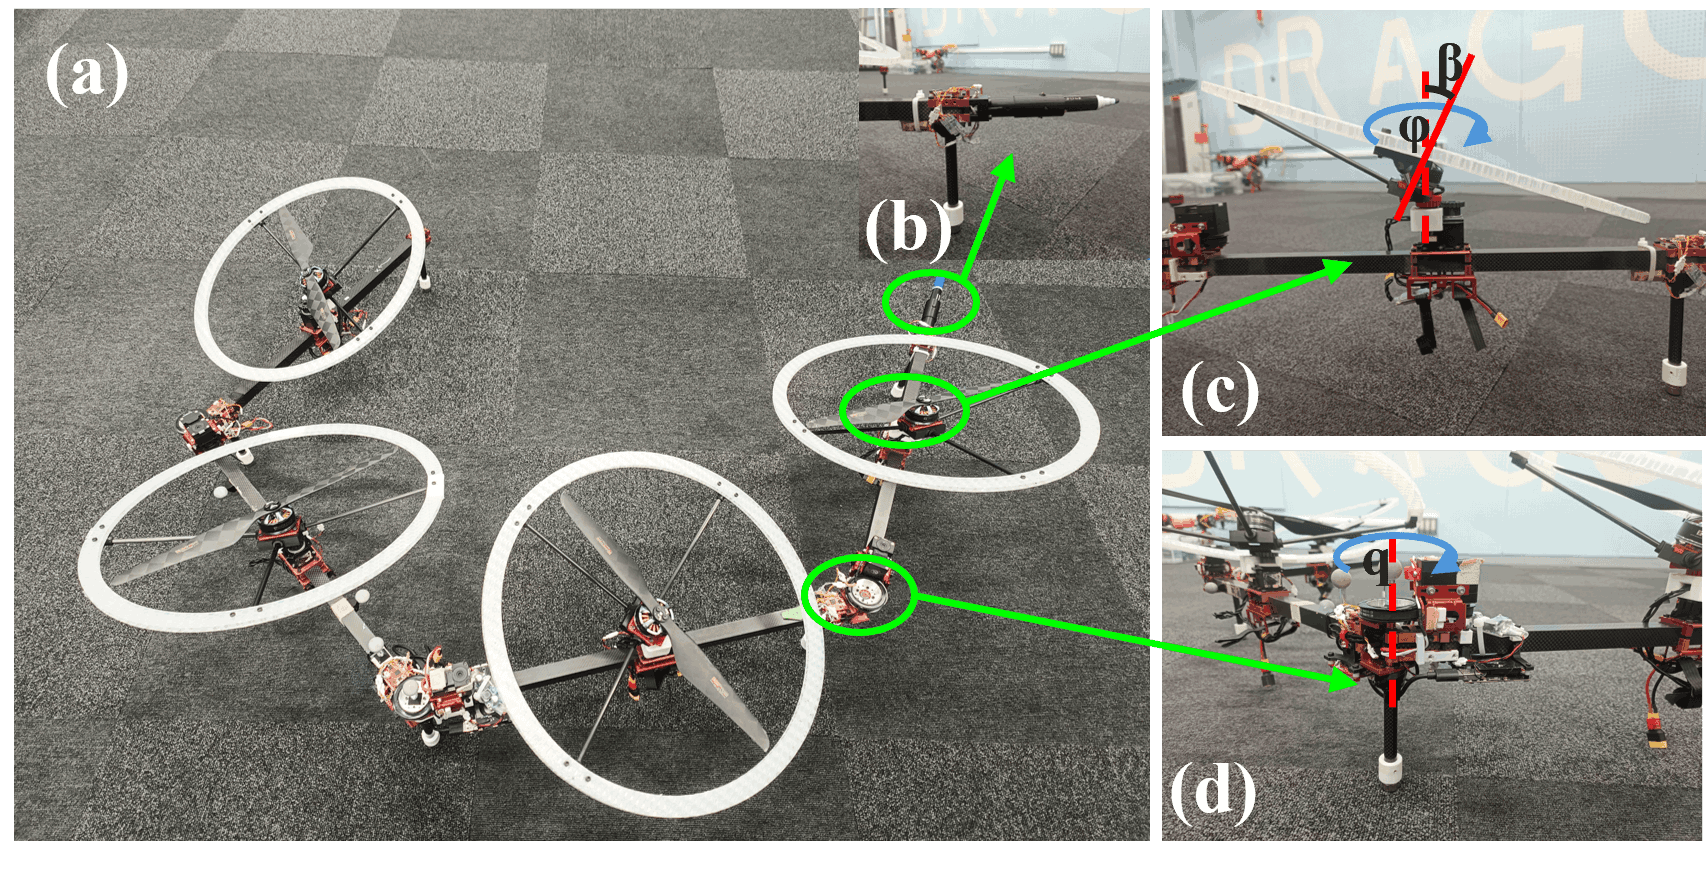
\includegraphics[trim={0cm 0cm 0cm 0cm}, clip, width=\linewidth]{figures/chapter6/robot_hydrus.png}
    \caption{The mechanical design of the 2D multi-link aerial robot Hydrus. (a) Overall mechanical structure. (b) End effector used in surface sliding experiments. (c) Gimbal module. (d) Joint.}
    \label{fig:robot_hydrus}
\end{figure}

\subsection{3D Multi-Link aerial robot DRAGON}
The 3D multi-link aerial robot DRAGON used in the experiments is shown in Fig.~\ref{fig:robot_dragon}. Similar to Hydrus Xi, DRAGON also consists of four serial links, but adjacent links are connected by two orthogonal joints, resulting in a total of six joint DoFs. Due to this robotic-arm-like mechanism, DRAGON can deform in three-dimensional space and achieve more complex configurations than Hydrus Xi. Each link is equipped with an independent gimbal module with two ducted rotors. The gimbal module provides 2-DoF to realize more flexible thrust vectoring thrust under complex deformations. The platform is equipped with an UP-Board single-board computer featuring an Intel Atom x7-Z8700 quad-core CPU for onboard computation.

\begin{figure}[!htbp]
    \centering
    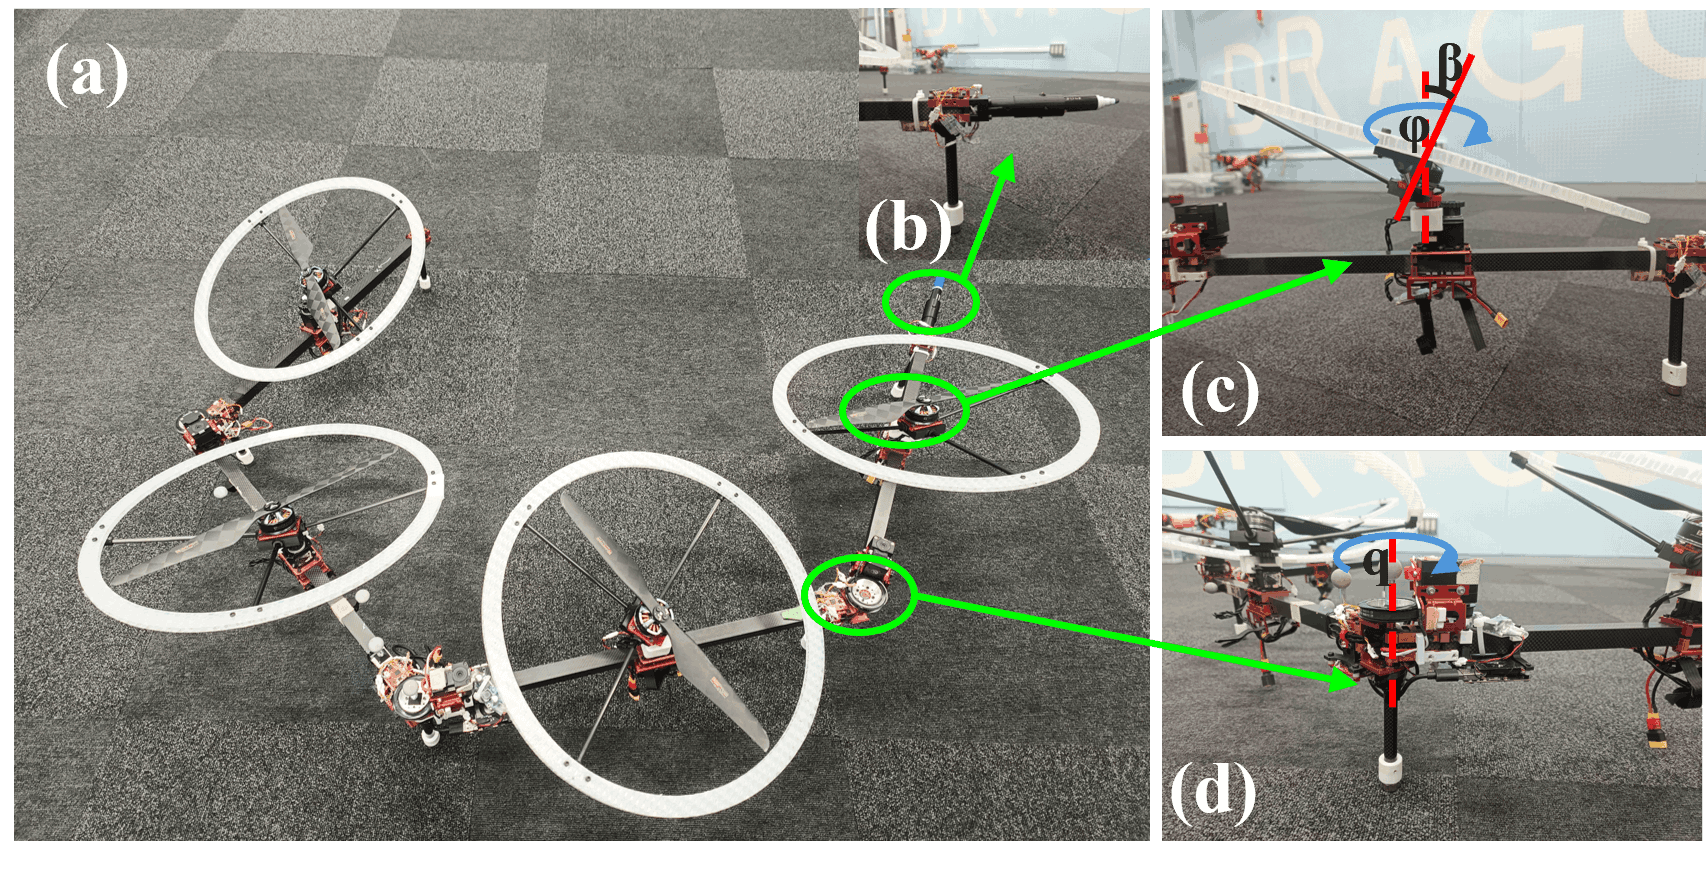
\includegraphics[trim={0cm 0cm 0cm 0cm}, clip, width=\linewidth]{figures/chapter6/robot_hydrus.png}
    \caption{The mechanical design of the 3D multi-link aerial robot DRAGON. (a) Overall mechanical structure. (b) End-effector used in surface sliding experiments. (c) Gimbal module. (d) Joints.}
    \label{fig:robot_dragon}
\end{figure}

%%%%%%%%%%%%%%%%%%%%%%%%%%%%%%%%%%%%%%%%%%%%%%%%%%%%%%%%%%%%%%%%%%%%%%%%%%%%%%%%
\section{Experimental parameters adjustment}
\subsection{Parameter Effects and Selection for Hydrus Xi}
\label{sec:parameter_selection}


In this work, the 2D mult-link aerial robot Hydrus Xi is used as the primary experimental platform, so that its controller parameters were selected according to the following practical considerations. These parameters will be tuned during preliminary experiments before conducting the main surface sliding experiments.

Since Hydrus Xi is an underactuated system, the rotational and translational parameters need to be tuned cascadely. Accoding to the principle mentioned in Sec~\ref{sec:imp_param_tuning}, the PD parameters are considered first. To achieve fast convergence to the desired orientation, $\tilde{c}_d$ in roll and pitch axes was set to a relatively large value. Meanwhile, to avoid oscillation, the damping ratio $\zeta$ in these two axes was tuned to approximately $1.2-1.4$. The remaining parameters were then adjusted according to the experimental conditions.

Next, the mass ratio $\mu$ in each direction needs to be taken into acconut. To reduce the influence of external torques on the orientation, the mass ratio $\mu$ in these directions was set relatively large, typically around $5-10$ in our experiments. For the translation directions, the selection depends on the task requirement. In the surface sliding task, it is usually need to contact in one direction and sliding in the other two directions as shown in Fig~\ref{fig:hybrid_controller}. In the sliding directions, it is imporant to resist to the friction-induced disturbances. Therefore. the $\mu$ is set larger than $1$,  typically around $1$--$3$ in our experiments. In the contact direction, only admittance behavior is required, while the impedance characteristic is not introduced. Therefore, $\mu$ is set exactly to $1$.

The admittance parameters were also selected based on the following principles. 

The admittance stiffness $k_a$ was mainly chosen according to the task requirement. If a large geometry variation is expected, a relatively small stiffness should be selected, and vice versa. Meanwhile, a larger stiffness results in less obvious deformation, whereas a smaller stiffness may introduce to a significant configuration variation that could lead to instability. Therefore, the admittance stiffess needs to be appropriately tuned according to the actual task conditions.

The admittance mass $m_a$ was selected mainly according to the required response speed. A larger admitttance mass results in a slower response, which may lead to insufficient adaptation to relatively fast geometric variations. On the other hand, a smaller admittance mass results in a faster respongse, which may introduce instability since the configuration may change too rapidly. In a word, the admittance mass also need to be appropriately tuned according to the task requirements.

Finally, the admittance damping $c_a$ was usually selected depend together with $m_a$ and $k_a$. The damping ratio $\zeta=\frac{c_a}{2\sqrt{m_ak_a}}$ was generally set slightly below $1$ to obtain a response close to critical damping.


\subsection{Free Flight Parameter Tuning}


According to the parameter tuning principle mentioned in Sec~\ref{sec:imp_param_tuning}, the PD parameters are first tuned under free flight conditions before introducing contact interaction. Note that in this stage, the mass ratio $\mu$ in all directions is set to $1$, such that no additional impedance characteristic is introduced. Meanwhile, the admittance controller is deactivated. Therefore, the controller in this experiment can be regarded as the baseline PD controller.

The parameters obtained from the free flight tuning are summarized in Table~\ref{tb:params1}.

\begin{table}[H]
    \centering
    \caption{Parameters for free flight.}
    \label{tb:params1}
    \begin{tabular}{ccc}
        \hline
        Name & Notation & Value \\
        \hline
        Normalized linear stiffness matrix & $\tilde{\boldsymbol{K}}_{td}$ & $diag(2.5, 2.5, 1.5)$ \\
        Normalized rotational stiffness matrix & $\tilde{\boldsymbol{K}}_{rd}$ & $diag(40.0, 40.0, 10.0)$ \\
        Normalized linear damping ratio matrix & $\boldsymbol{Z}_{td}$ & $diag(0.6, 0.6, 0.7)$ \\
        Normalized rotational damping ratio matrix  & $\boldsymbol{Z}_{rd}$ & $diag(1.1, 1.1, 0.8)$ \\
        \hline
    \end{tabular}
\end{table}
Here, the damping parameters are represented by the damping ratio instead of the damping coefficient. The corresponding damping matrices can be calculated as

\begin{subequations}
\label{eq:damping rate}
\begin{align}
\tilde{\boldsymbol{C}}_{td}&=2\boldsymbol{Z}_{td}\tilde{\boldsymbol{K}}^{\frac{1}{2}}_{td}, \\[2pt]
\tilde{\boldsymbol{C}}_{rd}&=2\boldsymbol{Z}_{rd}\tilde{\boldsymbol{K}}^{\frac{1}{2}}_{rd}.
\end{align}
\end{subequations}

The free flight result is shown in in Fig.~\ref{fig:free_flight_plot}. Here, the $z$ position and $yaw$ angle show relatively good tracking performance, whereas larger tracking errors can be observed in the $x$ and $y$ directions. Nevertheless, this experiment showed that under the impedance control framework, the overall flight of the multi-link aerial robot can remain stable. After the free flight tuning process, these tuned parameters will be used as the basic controller parameters for the following contact experiments.

\begin{figure}[!htbp]
    \centering
    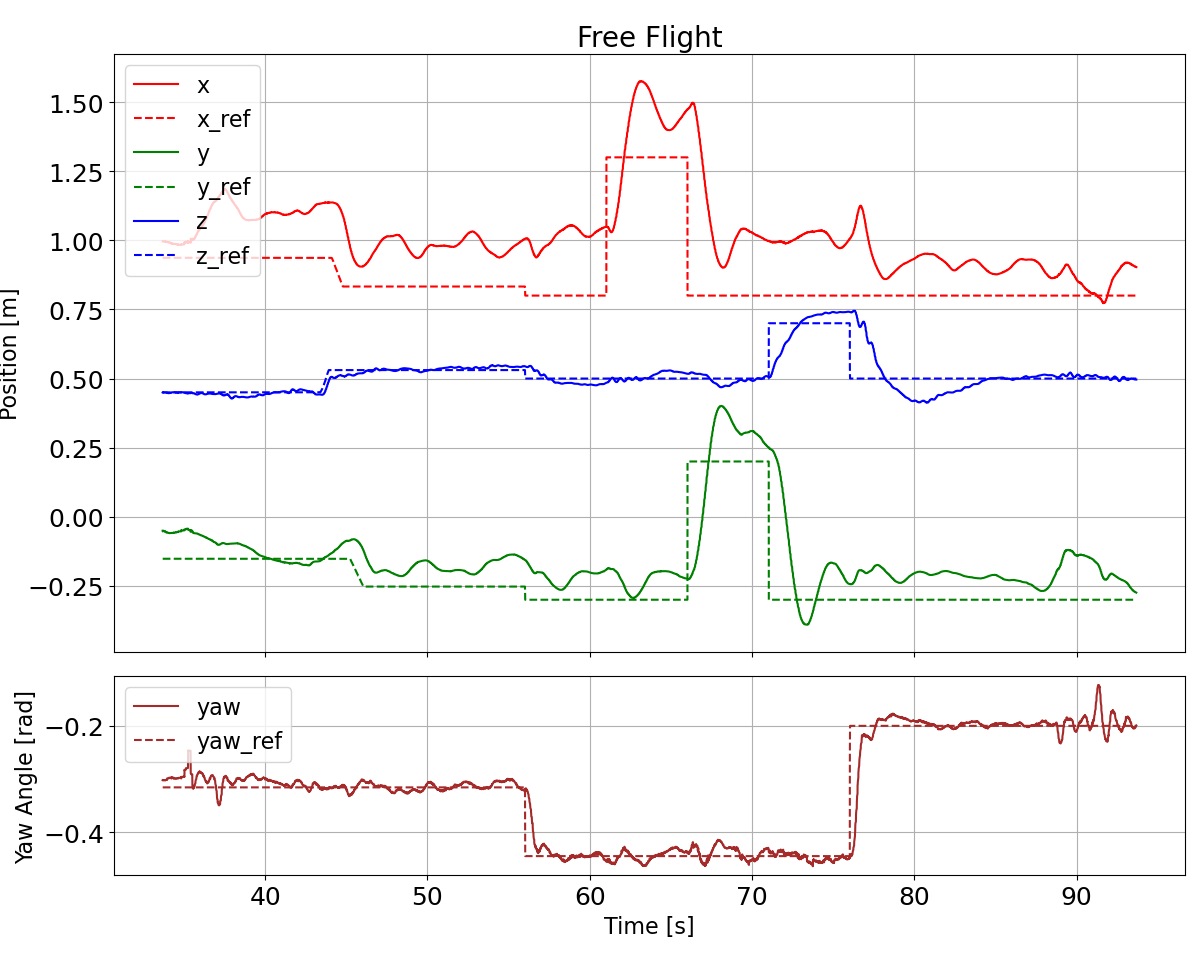
\includegraphics[trim={0cm 0cm 0cm 0cm}, clip, width=\linewidth]{figures/chapter6/free_flight_plot.png}
    \caption{Free flight response Hydrus Xi with the tuned PD parameters. The mass ratio $\mu$ in each direction is set to $1$, so that the impedance controller is reduced to a PD controller.}
    \label{fig:free_flight_plot}
    \vspace{-5mm}
\end{figure}

\subsection{Impedance Parameter Adjustment under External Force}

In this experiment, the effect of the mass ratio $\mu$ will be investigated. Accoding to Sec.~\ref{sec:imp_param_tuning}, the mass ration $\mu$ will redesigned the performance. In particular, $\mu>1$ provides a more rigid response to external disturbances, whereas $\mu<1$ provides a softer response.


As shown in Fig.~\ref{fig:imp_drag}, a rope is used to horizontally drag Hydrus Xi and generate an external force along the $x$ axis. Pulling the rope along the positive direction of the $x$ axis can be regarded as applying a positive external force along this direction. The other controller parameters are kept the same as those used in the free flight experiment, as listed in Table~\ref{tb:params1}. Three different mass ratios, $\mu=0.5$, $1$, and $2$, are tested, corresponding to the soft, normal, and rigid cases, respectively. 


% we will do a experiment to valid the ability of impedance control. We can demonstrate that by varifying the parameter $\mu$, the performance of multi-link aerial robot will become different.


% Here we will measure the estimated external force in $x$ axis and the corresponding CoG displacement in $x$ axis. The result is shown in Fig. \ref{fig:drag_plot}. In the analysis in Sec, when $\mu$ is larger than $1$, the system can be considered as a rigid system. On the other hand,  when $\mu$ is smaller than $1$, the system can be considered as a soft system.



\begin{figure}[!htbp]
    \centering
    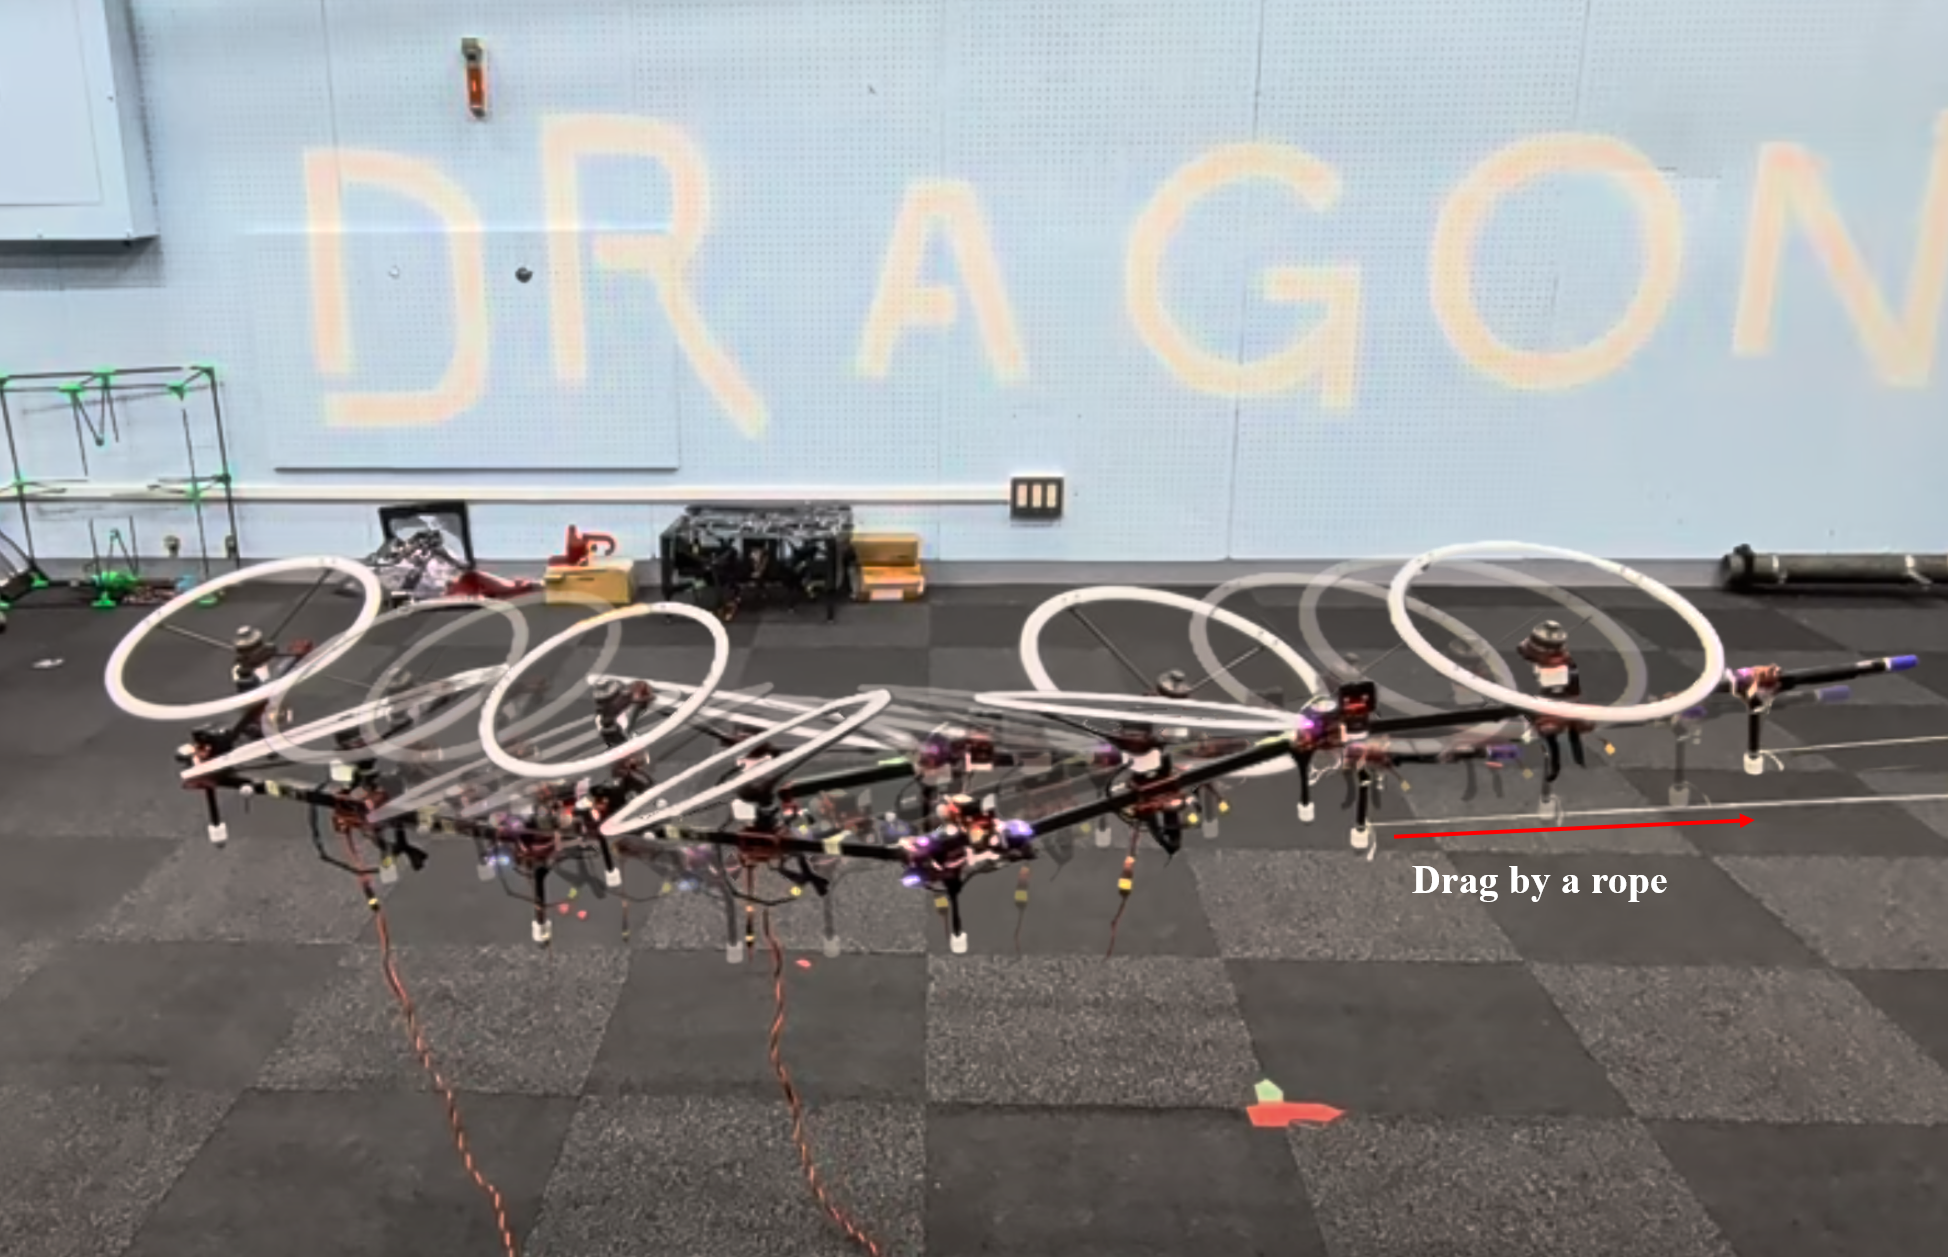
\includegraphics[trim={0cm 0cm 0cm 0cm}, clip, width=\linewidth]{figures/chapter6/imp_drag.png}
    \caption{The multi-link aerial robot is dragged by a rope to simulate the external force on a single direction. The aerial robot move in order to generate enough consistant force to the external dragging force along the $x$ axis.}
    \label{fig:imp_drag}
\end{figure}

As illustrated in Fig.~\ref{fig:imp_drag_result}, during the experiment, Hydrus Xi is gradually dragged away from its reference position until larger position error becomes hard to achieve. A larger position error can be observed in the soft case, whereas the rigid case exhibits a smaller position error. Although the same external force is not guaranteed in different cases, the results intuitively show that a larger $\mu$ leads to a more rigid response, and demonstate that the impedance controller can modify the dynamic performance of the multi-link aerial robot.



\begin{figure}[!htbp]
    \centering
    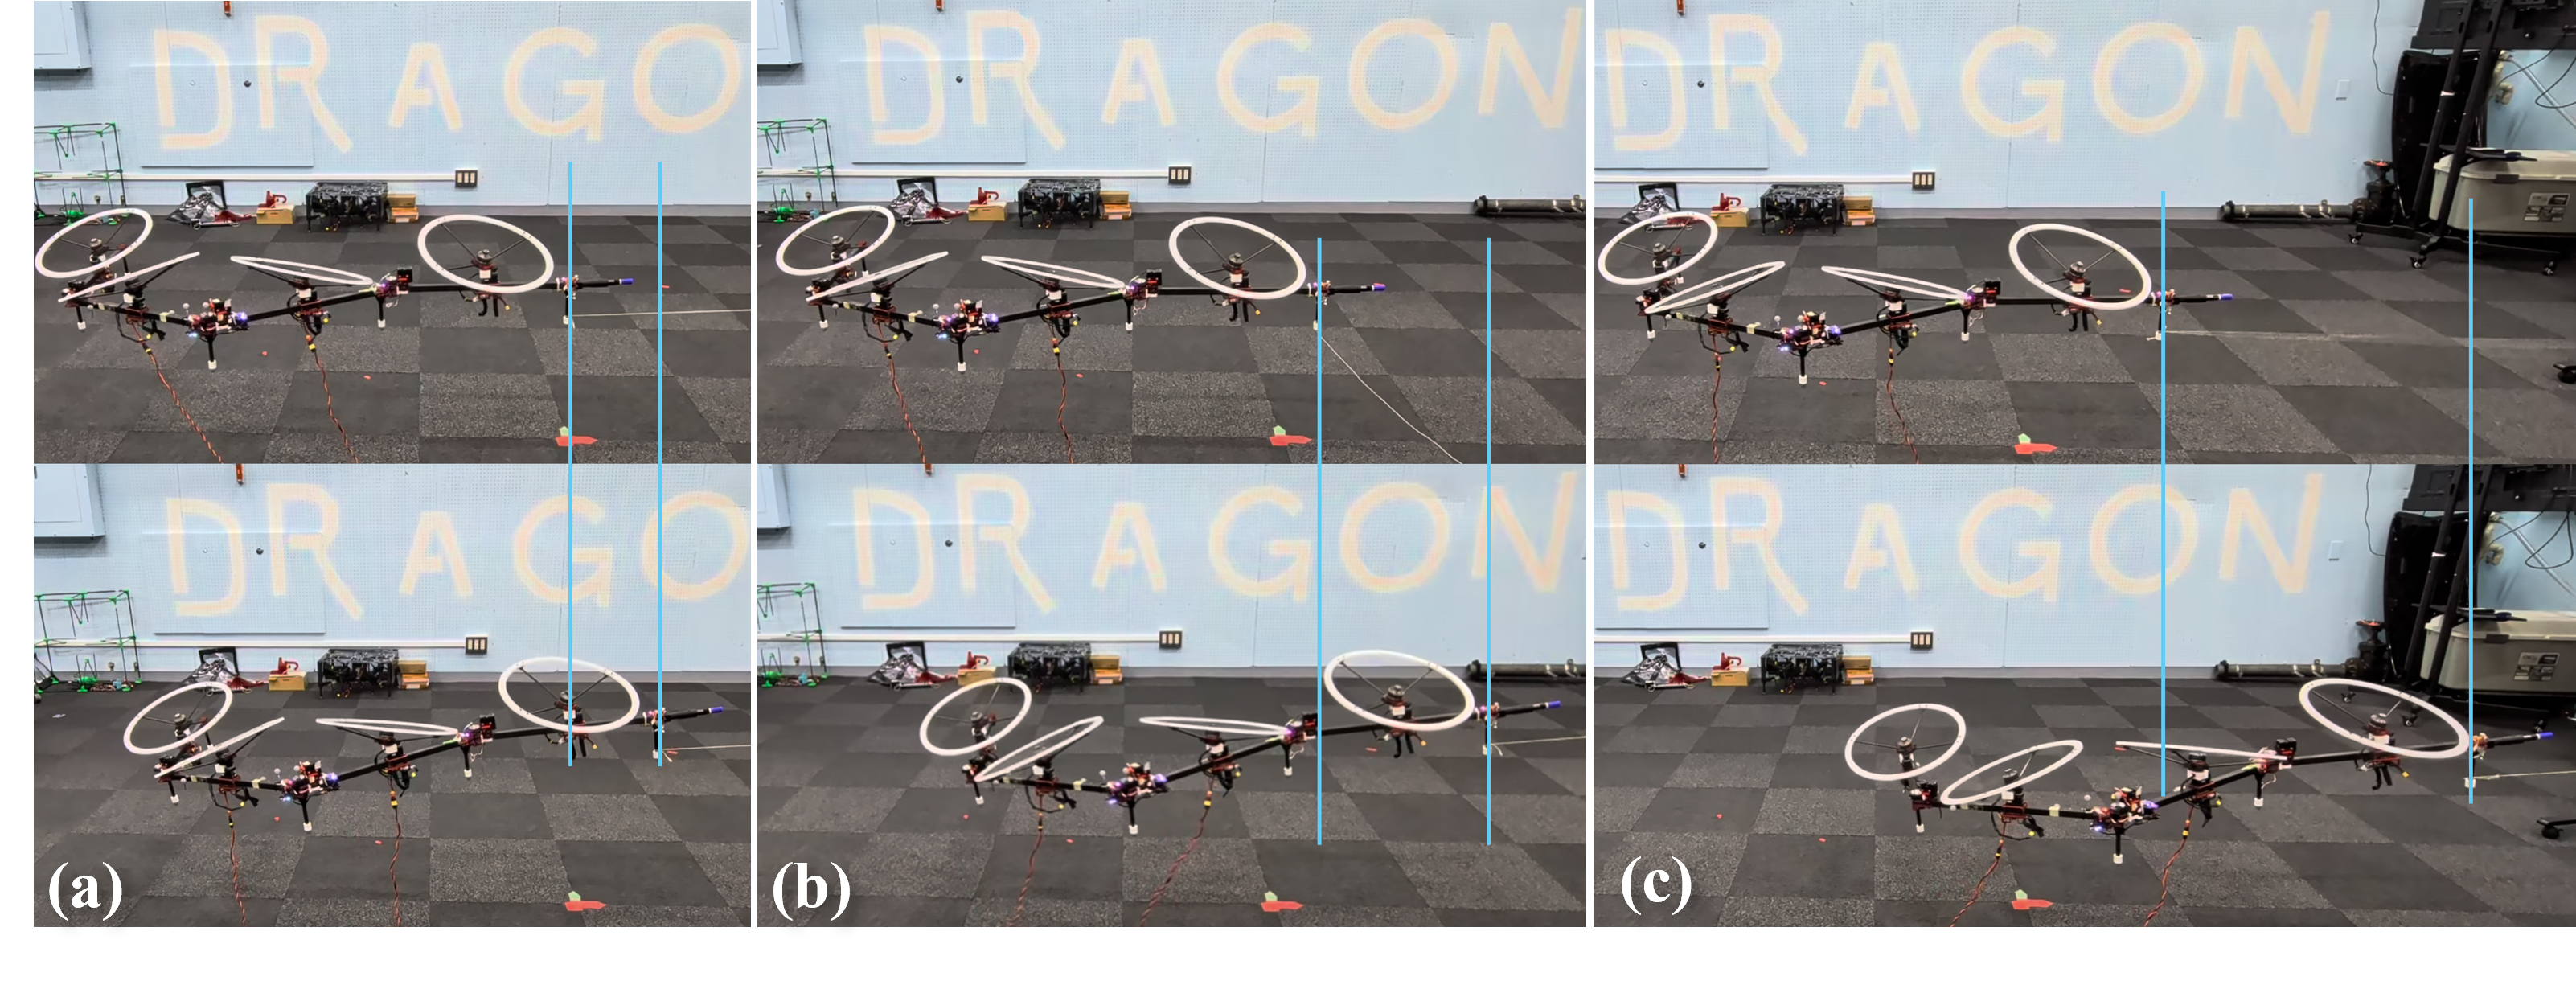
\includegraphics[trim={0cm 0cm 0cm 0cm}, clip, width=\linewidth]{figures/chapter6/imp_drag_result.png}
    \caption{Results of the dragging experiment with different mass ratios: (a) rigid case ($\mu = 2$). (b) normal case ($\mu = 1$). (c) soft case ($\mu = 0.5$).}
    \label{fig:imp_drag_result}
\end{figure}


\begin{figure}[!htbp]
    \centering
    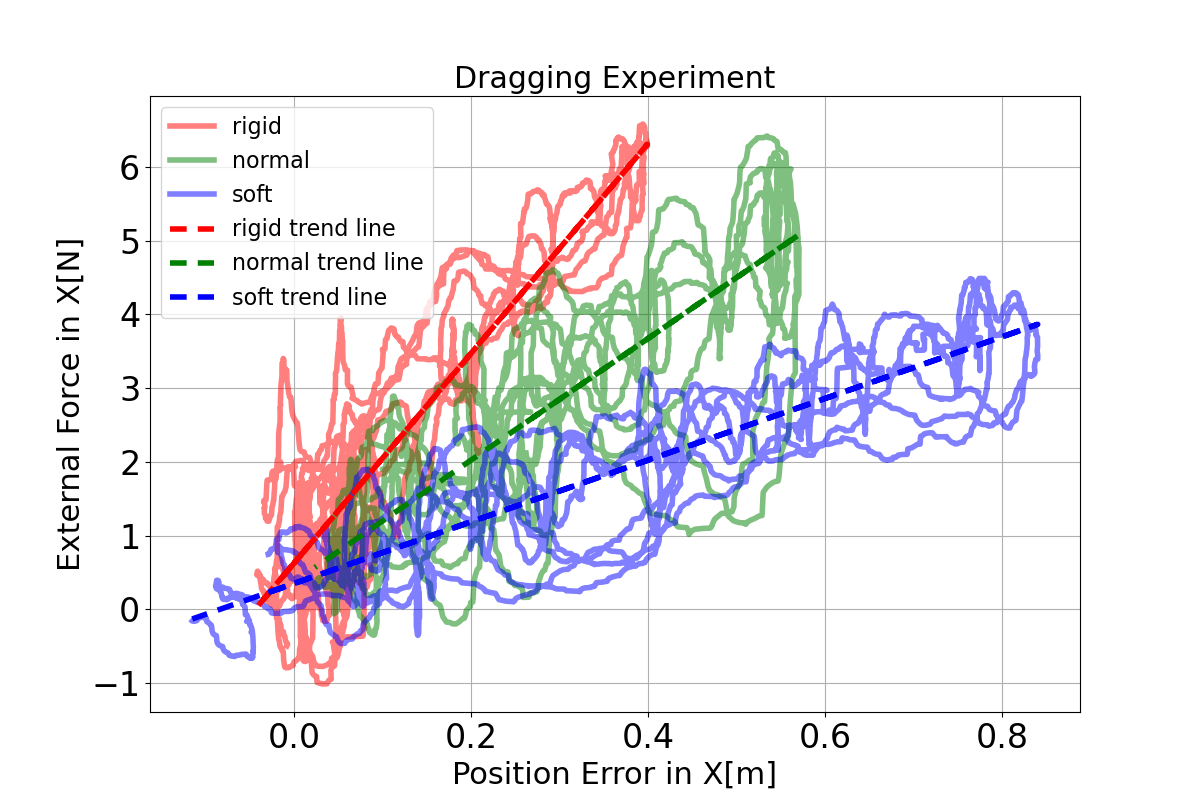
\includegraphics[trim={0cm 0cm 0cm 0cm}, clip, width=\linewidth]{figures/chapter6/imp_drag_plot.png}
    \caption{The plot of the dragging experiment, which shows the relationship between the estimated external force and the CoG position error in the dragging experiment with different mass ratios.}
    \label{fig:imp_drag_plot}
\end{figure}


The result in Fig.\ref{fig:imp_drag_plot} shows the relationship between the estimated external force and the CoG position error along the $x$ axis. The slope of the force-position relationship can be regarded as the effective stiffness. As shown by the trend line, the slopes for $\mu=0.5$, $1$, and $2$ are $4.18~\mathrm{N/m}$, $8.25~\mathrm{N/m}$, and $14.22~\mathrm{N/m}$, respectively. Consquently, the results demostrate that by varying the mass ratio $\mu$, the aerial robot could change its performance to the external force. Therefore, an appropriate mass ratio can be selected according to the experimental conditions and task requirements.


\subsection{Admittance Control under External Force}

In this experiment, the deformation behavior generated by the admittance controller is demonstrated using the 2D multi-link aerial robot Hydrus Xi. As shown in Fig.~\ref{fig:admittance_drag}, Hydrus Xi starts from its nominal configuration, which a rope attach at one of the joints. By pulling the rope to the negative direction of the $x$ axis, an external force on the negative direction of the $x$ axis can be imitated. We need to emphasize that in this and the following experiments, as shown in Fig.~\ref{fig:admittance_drag}, the distance $r$ used in admittance controller \ref{eq:admittance control2} is defined as the distance between the end effector and the CoG projected onto the $x$ axis.


The admittance parameters were selected according to the practical considerations introduced in Sec.~\ref{sec:parameter_selection}. The purpose of this experiment is to demonstrate the structural deformation induced by the admittance controller under an external force.


\begin{figure}[!htbp]
    \centering
    % \parbox{3in}
    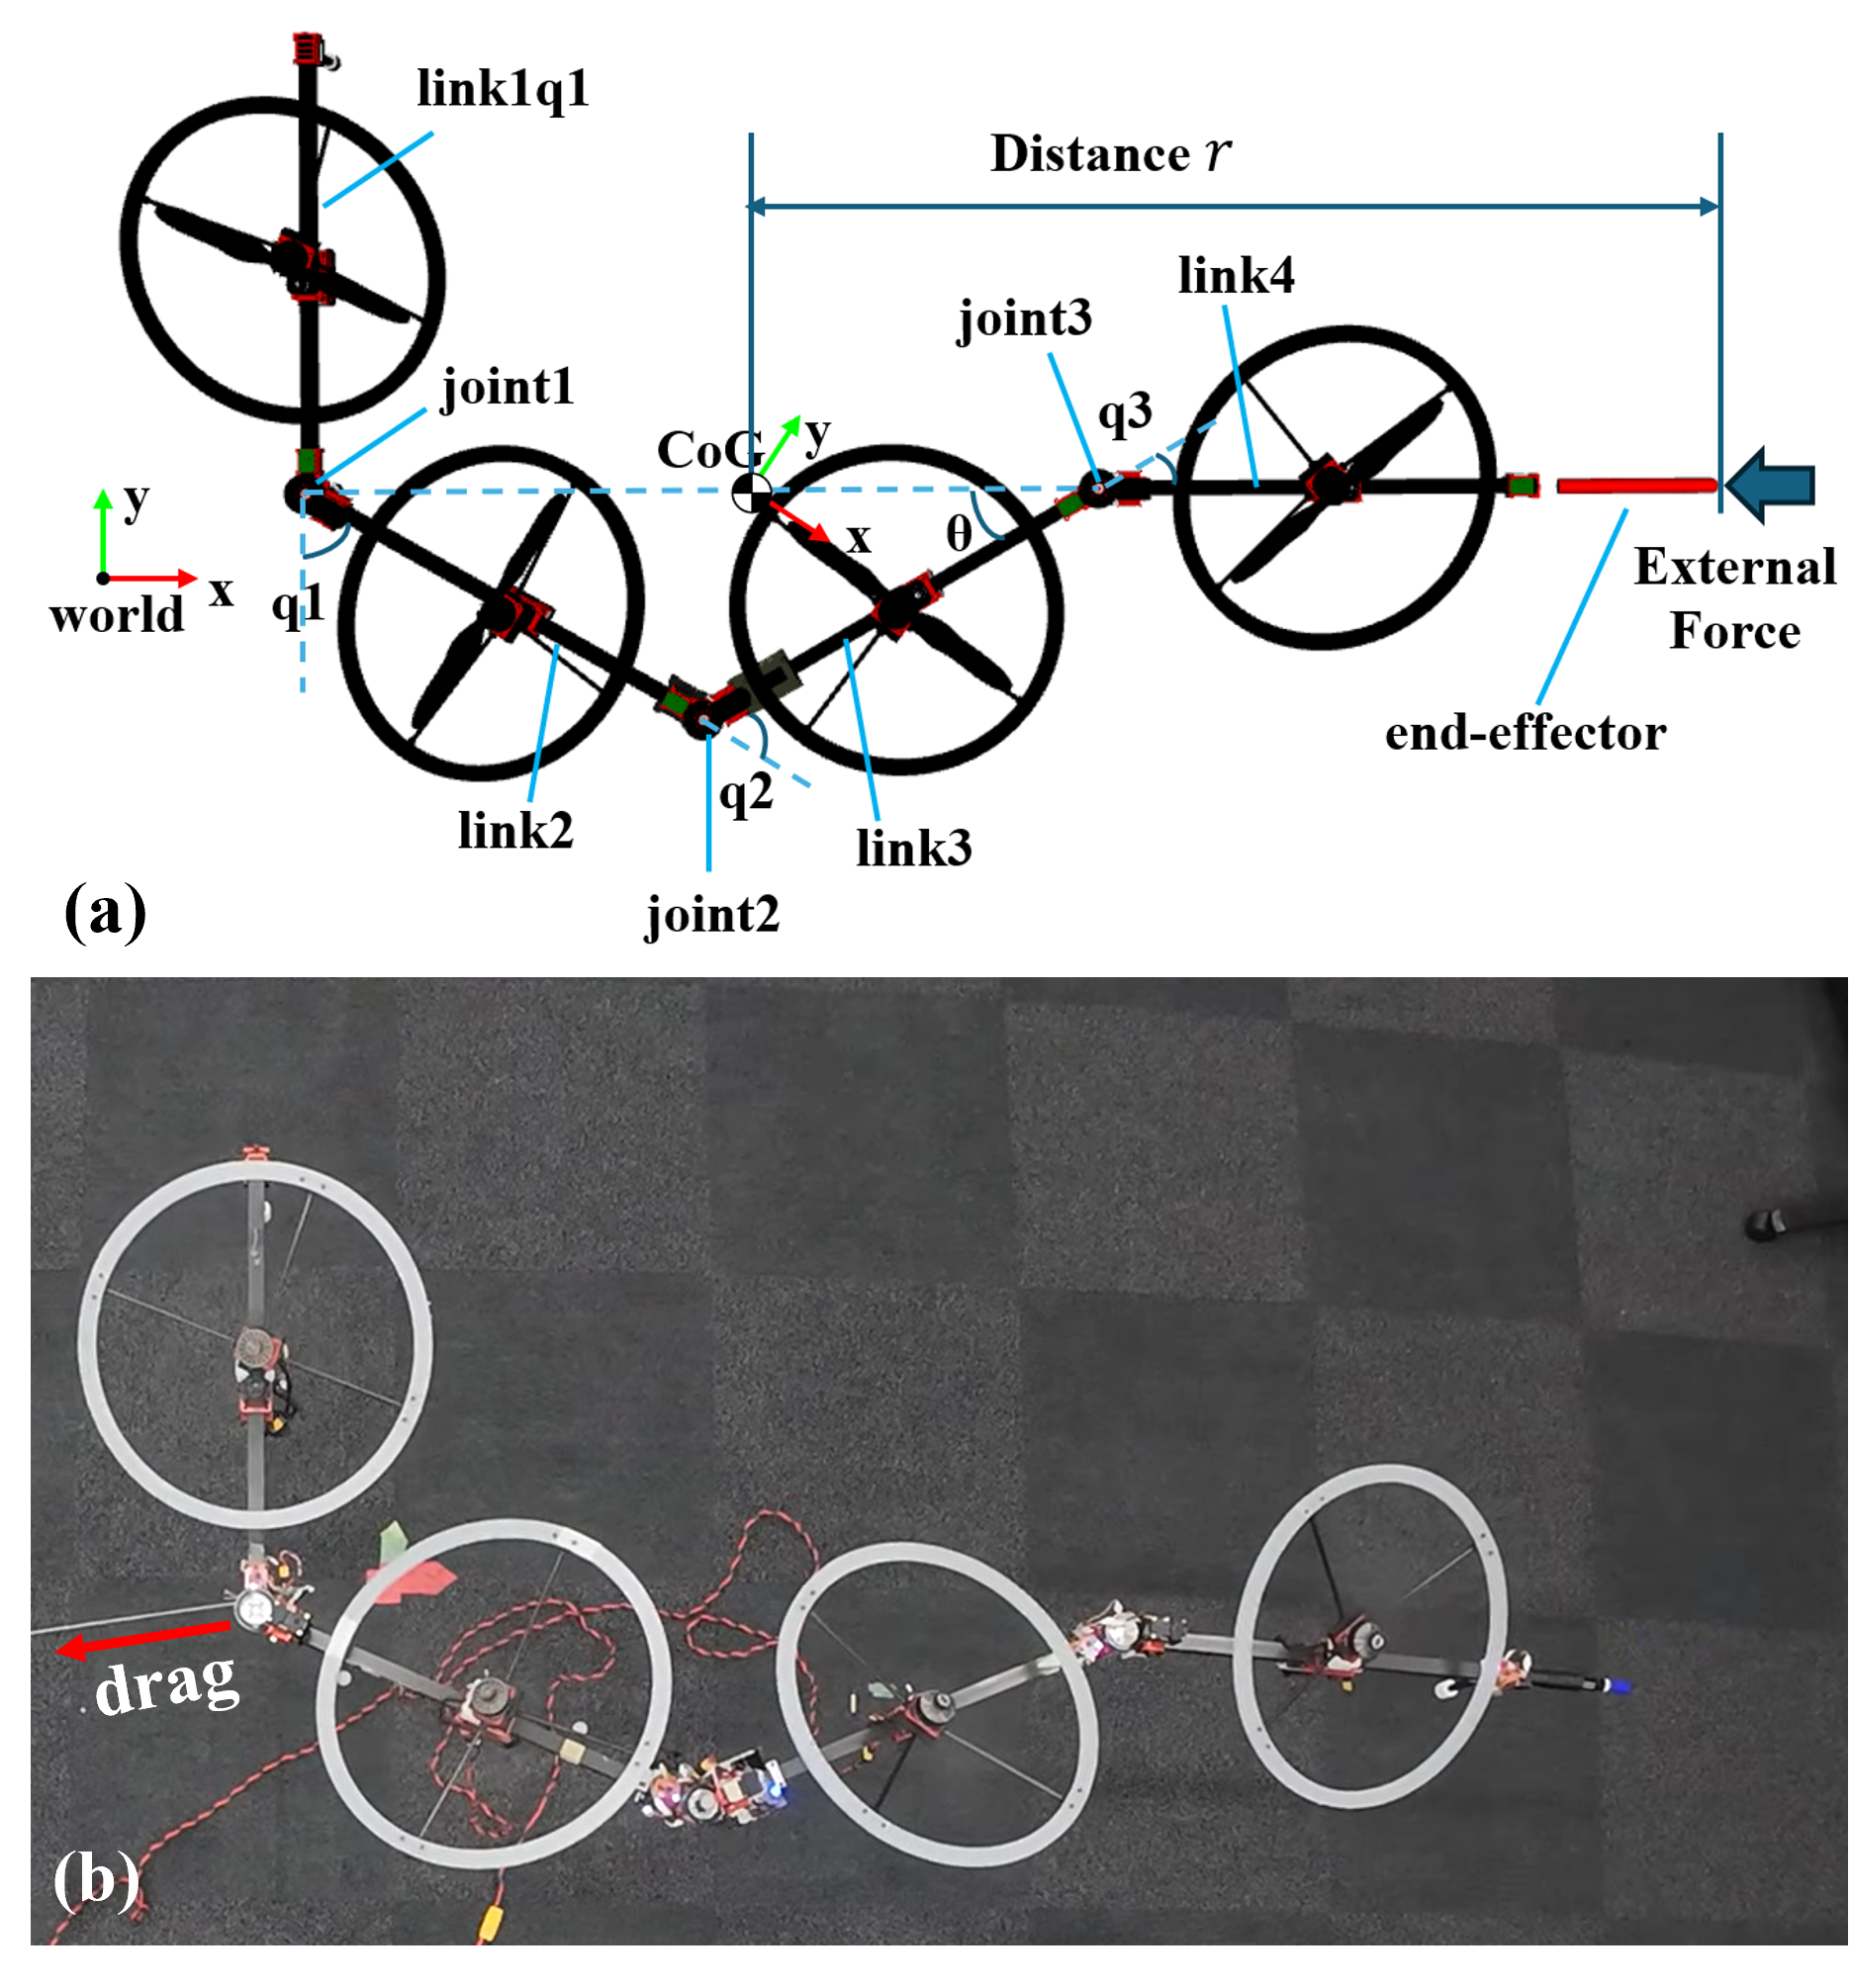
\includegraphics[trim={0cm 0cm 0cm 0cm},clip,width=\linewidth]{figures/chapter6/admittance_drag.png}
    \caption{(a) The nominal surface-contact configuration of the multi-link aerial robot. The distance used in admittance controller is shown as the distance between the end effector and the CoG along the $x$ axis of $\{W\}$. The configuration angle $\theta = \pi /6$, and the joint angles $q_1$, $q_2$, $q_3$ are consequently $\pi /3, \pi /3,-\pi /6$, respectively. (b) The aerial robot is dragged by the rope to imitate the exteral force added on the $x$ axis.}
    \label{fig:admittance_drag}
\end{figure}



As shown in Fig.~\ref{fig:admittance_changing}, the multi-link structure changes in response to the applied external force. The snapshots provide a visualization of the deformation process under the admittane controller. The relationship among the external force, the end effector--CoG distance, and the joint angles is shown in Fig.~\ref{fig:admittance_deformation_plot}. During the interval indicated by the pink region, the admittance controller is activated and the multi-link aerial robot is dragged along the negative direction of $x$ axis. The estimated external force along the $x$ axis consequently shows an apparent negative value, and the end effector--CoG distance varies in response to the external force. Through the inverse kinematics, the variation in distance is further converted into changes in the joint angles, resulting in deformation of the multi-link structure. This result demonstrates that the multi-link aerial robot could deformation under external force on the admittance controller activated direction.


% Here we define the length of each link as $l$, the length of end effector is $d$, the mass of every link (with the propeller module) as $m_i, i \in {1, 2, 3, 4}$. We can cauculte the value $\theta$ as follow:

% \begin{equation}
% \label{eq:distance2joint}
% cos\theta = (r-d-l)/4
% \end{equation}

% After getting the $\theta$ .Note that the distance $r$ is constr between $1.08 m$ in order to avoid out range.

\begin{figure}[!htbp]
    \centering
    % \parbox{3in}
    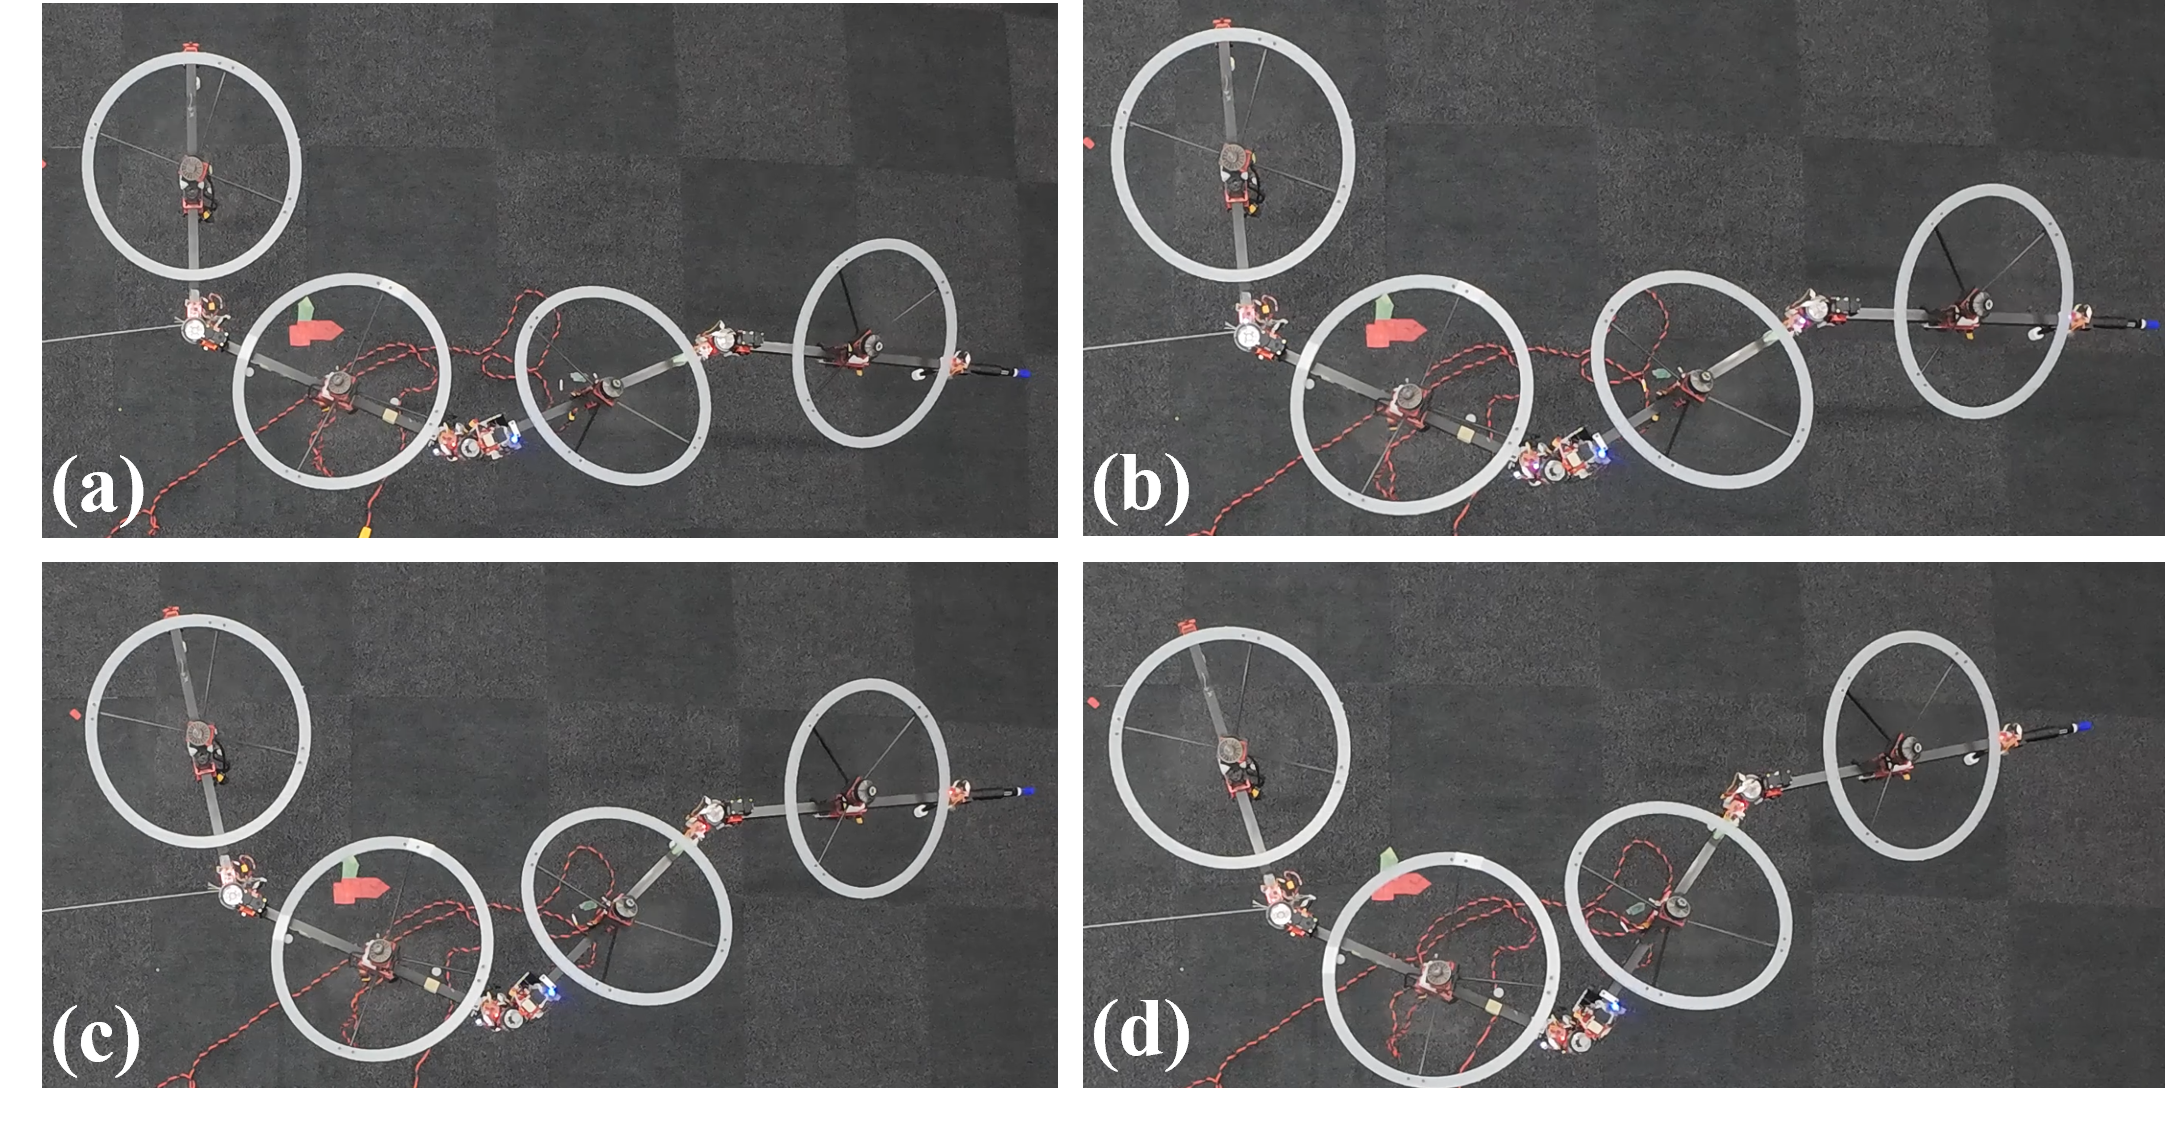
\includegraphics[trim={0cm 0cm 0cm 0cm},clip,width=\linewidth]{figures/chapter6/admittance_changing.png}
    \caption{Snapshots of the top view of the multi-link aerial robot, in which the deformation under admittance control can be observed. (a)--(d) show the deformation process of the multi-link aerial robot in response to the pulling force applied through the rope.}
    \label{fig:admittance_changing}
\end{figure}


\begin{figure}[!htbp]
    \centering
    % \parbox{3in}
    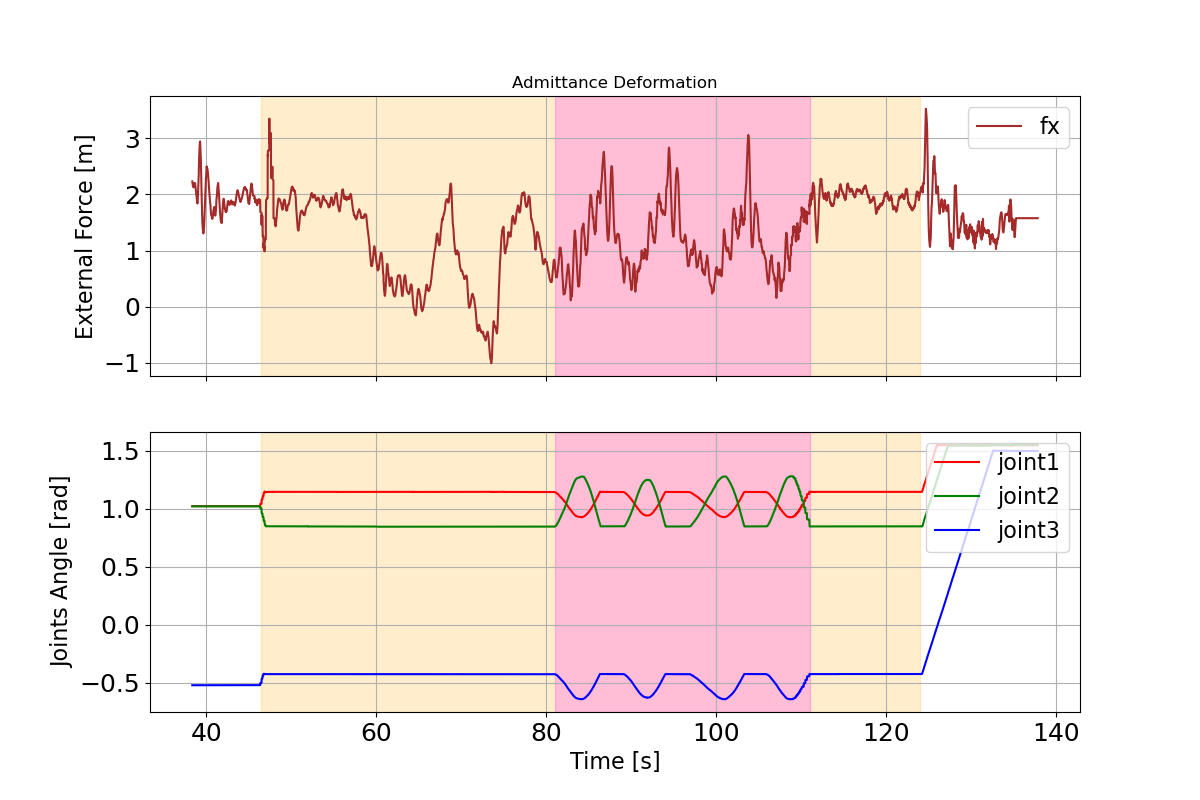
\includegraphics[trim={0cm 0cm 0cm 0cm},clip,width=\linewidth]{figures/chapter6/admittance_deformation_plot.png}
    \caption{Plot about the external force acting on the CoG along the $x$ axis, the distance between the end effector and the CoG projected onto the $x$ axis, and joint-angle variations. The yellow region denotes the activation period of the admittance controller, and the pink region indicates the interval during when the aerial is dragged by the rope.}
    \label{fig:admittance_deformation_plot}
\end{figure}





% In this experiment, we use a rope to horizontally drag the multi-link aerial robot in order to imitate the horizontal external force. The dragging direction is similar to the impedance part. The other parameters are shown in the following Table \ref{tb:params3}.

% Here we measure the estimated external force in X axis and the corresponding displacement in X axis. The result is shown in Fig.\ref{fig:drag_plot2}.


% The experiment result varify that the distance between CoG and end-effector can change with the external force. By setting parameters like this, we can guarantee stability and response speed, simultaneously
% \subsection{Hybrid control}
% In this section, we show that the hybrid impedance-admittance controller can be used in the multi-link aerial robot. As shown in Fig.\ref{fig:hybrid_showing}, the robot realize consist to the friction and adapt to the surface variation, simultaneously.


%%%%%%%%%%%%%%%%%%%%%%%%%%%%%%%%%%%%%%%%%%%%%%%%%%%%%%%%%%%%%%%%%%%%%%%%%%%%%%%%
\section{Hybrid Control Experiment on Hydrus Xi}
\subsection{Experimental Setup}


The actual experimental parameters are also same as the Table\ref{tb:params1}. Note that in $x$ axis, $\mu$ is chosen as $1$ so the impedance controller only performs PD part in this direction. Meanwhile, the admittance controller is only acting at $x$ axis, and the reference external force used in admittance controller is given by $f_{ref,x} = 0$. The other used parameters are shown in Table\ref{tb:params4}.
% as follows. The estimator translation and rotation gain matrices are given by $\boldsymbol{K}_{ti}=diag(3.0, 3.0, 3.0)$ and $\boldsymbol{K}_{ri}=diag(1.0, 1.0, 1.0)$. We treat $\boldsymbol{M}_d/m$ and $\boldsymbol{I}_d\boldsymbol{I}^{-1}$ as entities. Their values are set to $\boldsymbol{M}_d/m=diag(1.0, 3.0, 1.0)$, $\boldsymbol{I}_d\boldsymbol{I}^{-1}=diag(10.0, 10.0, 5.0)$. By choosing these values greater than $1$, the impedance controller exhibits more resilient behavior against environmental disturbances due to the increased designed stiffness. The normalized linear stiffness and rotational stiffness are given by $\tilde{\boldsymbol{K}}_{td} = diag(2.5, 2.5, 1.5)$, $\tilde{\boldsymbol{K}}_{rd} = diag(40.0, 40.0, 10.0)$. The normalized linear and rotational damping terms are not directly specified. Instead, we define the linear damping ratio $\boldsymbol{Z}_{td}=diag(0.6, 0.6, 0.7)$ and the rotational damping ratio $\boldsymbol{Z}_{rd}=diag(1.1, 1.1, 0.8)$, and compute the corresponding normalized damping matrices as follows:


\begin{table}[H]
    \centering
    \caption{Parameters of surface sliding experiment.}
    \label{tb:params4}
    \begin{tabular}{lcc}
        \hline
        Name & Notation & Value \\
        \hline
        Estimator translation gain matrix & $\boldsymbol{K}_{ti}$ & $diag(3.0, 3.0, 3.0)$ \\
        Estimator rotation gain matrix & $\boldsymbol{K}_{ri}$ & $diag(1.0, 1.0, 1.0)$ \\
        Linear mass ratio matrix & $\boldsymbol{M}_d/m$ & $diag(1.0, 3.0, 1.0)$ \\
        Inertia ratio matrix & $\boldsymbol{I}_d\boldsymbol{I}^{-1}$ & $diag(10.0, 10.0, 5.0)$ \\
        Admittance mass & $m_a$ & 40 \\
        Admittance damping & $c_a$ & 55 \\
        Admittance stiffness & $k_a$ & 16 \\
        \hline
    \end{tabular}
\end{table}

% \begin{figure}[t]
%      \centering
%     % \parbox{3in}
%     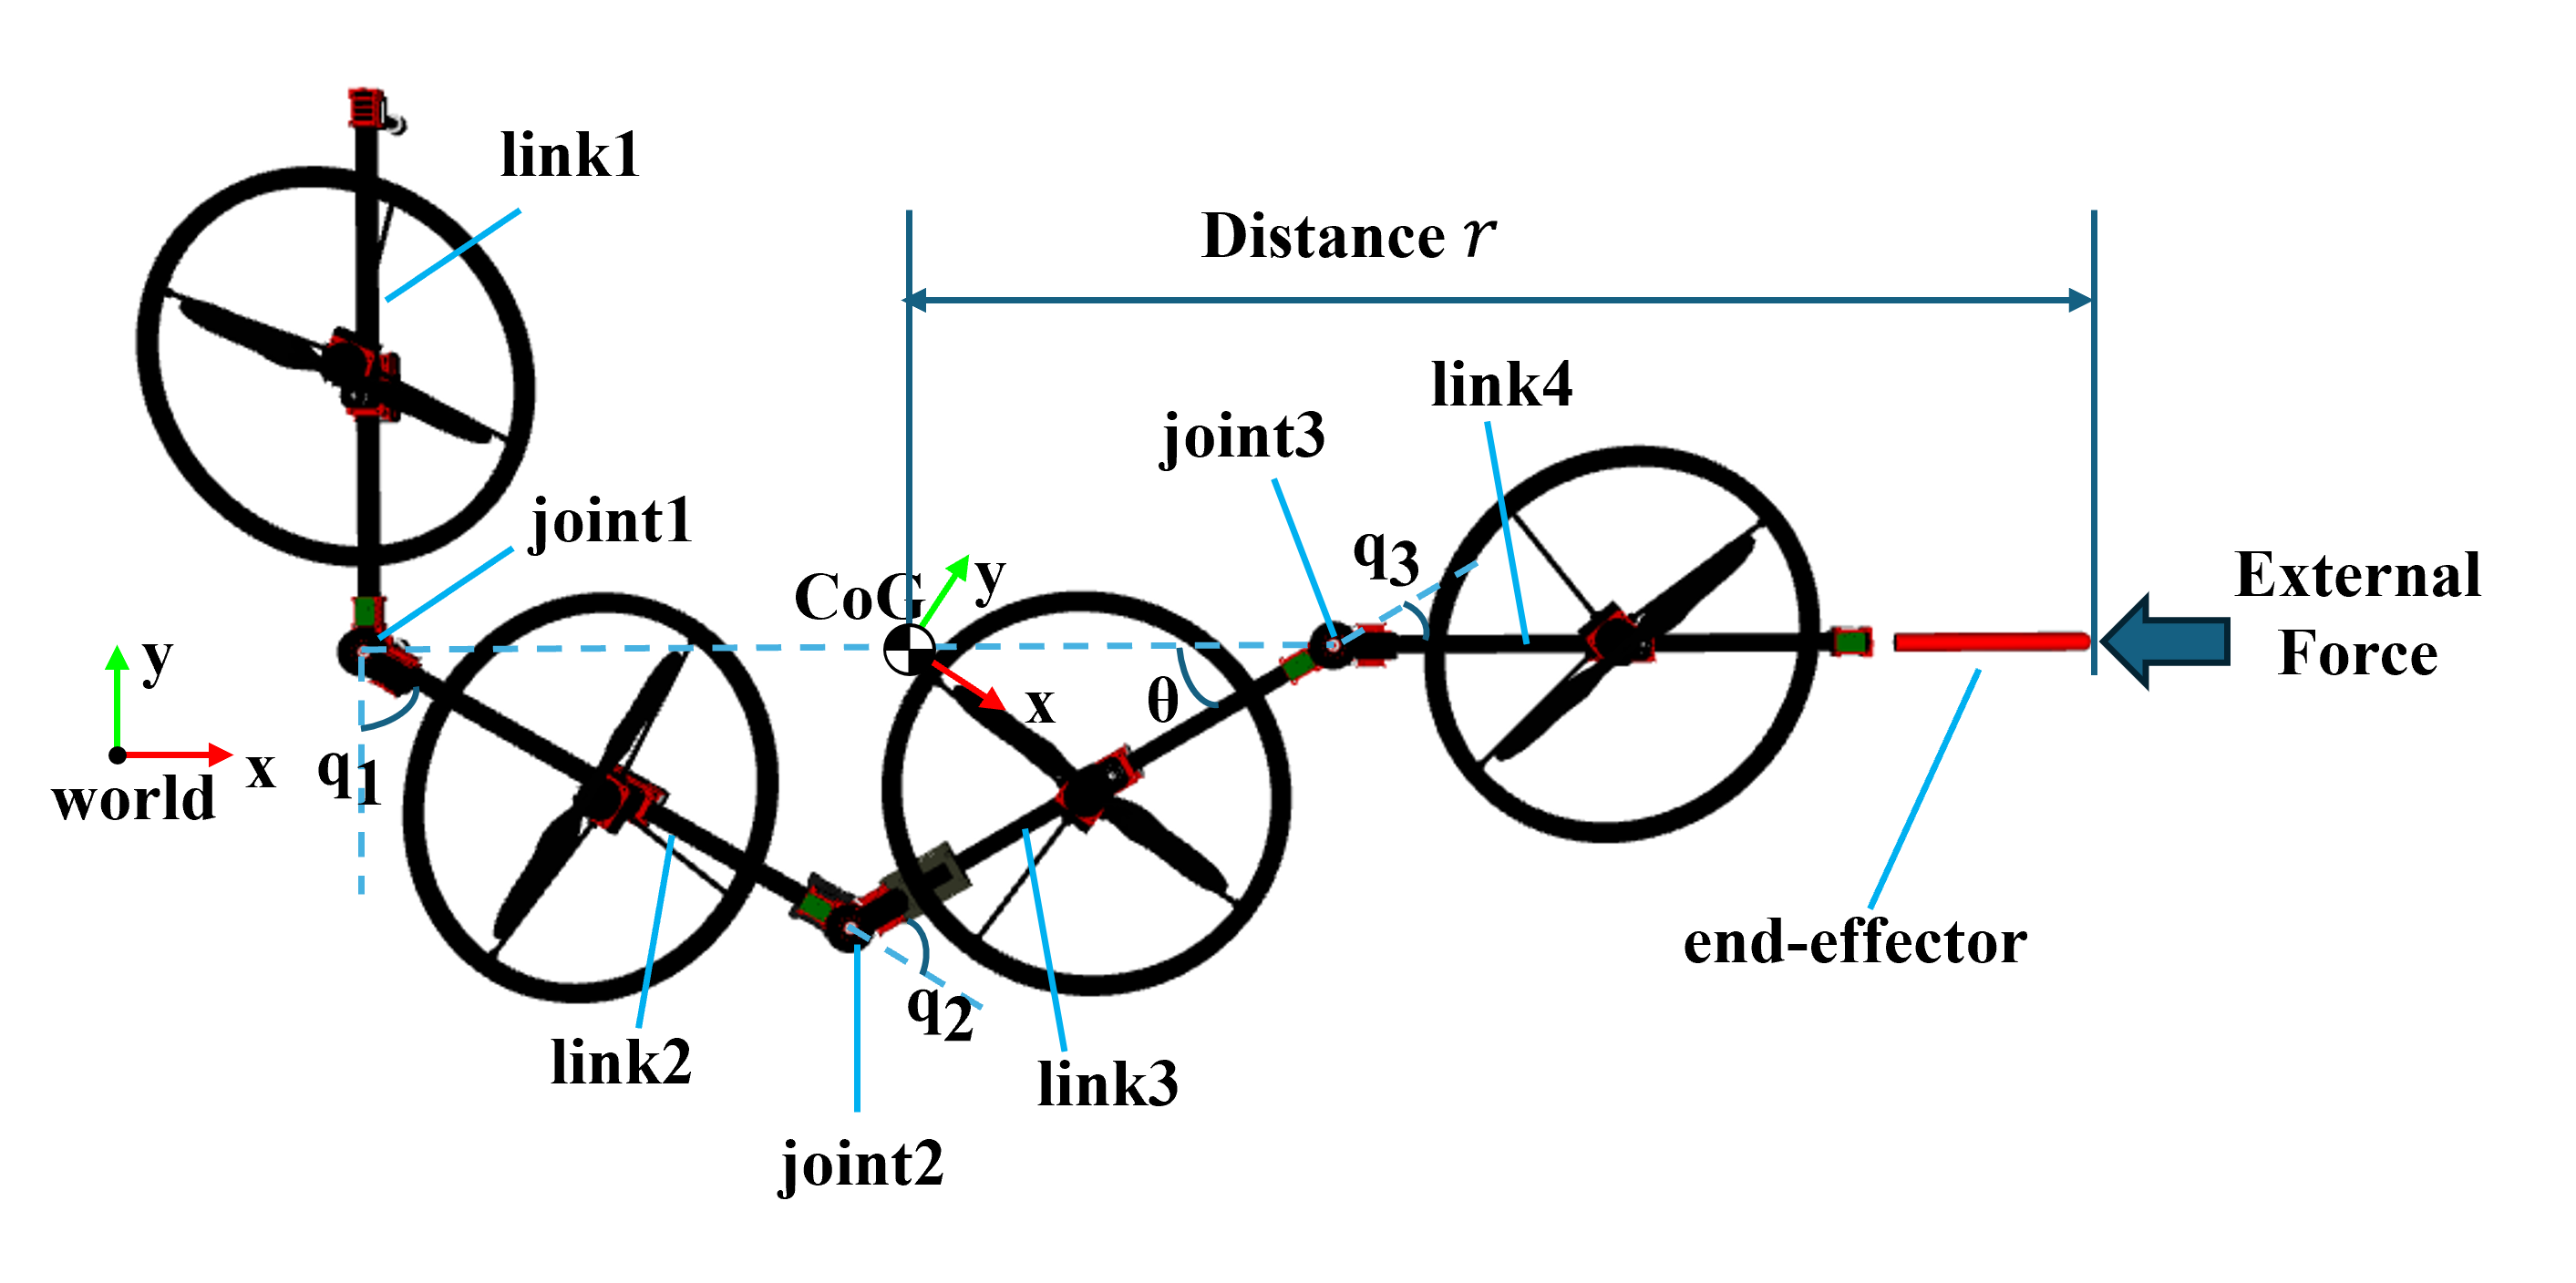
\includegraphics[trim={0cm 0.5cm 0cm 0cm}, clip, width=\linewidth]{figures/chapter5/hydrus.png}
%     \caption{The nominal surface-contact configuration of the multi-link aerial robot. The configuration angle $\theta = \pi /6$, and the joint angles $q_1$, $q_2$, $q_3$ are consequently $\pi /3, \pi /3,-\pi /6$, respectively.}
%     \label{fig:admittance control}
%     \vspace{-5mm}
% \end{figure}

Throughout the experiment, a constant yaw angle was commanded, implemented by keeping link 4 aligned with the $x$ axis in order to reduce external torque applied on the CoG. Specifically, here we defined the configuration angle $\theta$ as the variable in the admittance controller to determine the configuration solely and then computed the corresponding joint angles analytically through inverse kinematics. The angle of each joint was satisfied as

\begin{equation}
\label{eq:joint angles}
 \begin{bmatrix}
    q_1 \\
    q_2 \\
    q_3
    \end{bmatrix} 
    =
    \begin{bmatrix}
    \frac{\pi}{2}-\theta \\
    2\theta \\
    -\theta
    \end{bmatrix},
\end{equation}
where $\theta$ is shown in Fig.~\ref{fig:admittance_drag}.

The experimental environment is illustrated in Fig.~\ref{fig:exp_scene}. A vertical board was placed at a known location within the testing area. The board's surface provided sufficient friction for stable contact while still allowing smooth sliding of the end-effector (marker pen). The board's surface was intentionally sloped by approximately $20^\circ$ with respect to the $y$ axis, and the inclination angle was kept unknown to the robot. Although the surface is planar, its unknown inclination introduces unmodeled geometric variations that serve the same role as curved surfaces in this study. The friction coefficient is also unknown. Consequently, both the contact forces and the surface geometry remain unmodeled in this experiment, which provides a challenging benchmark for evaluating the robot's adaptive sliding capability.

\begin{figure}[!htbp]
    \centering
    % \parbox{3in}
    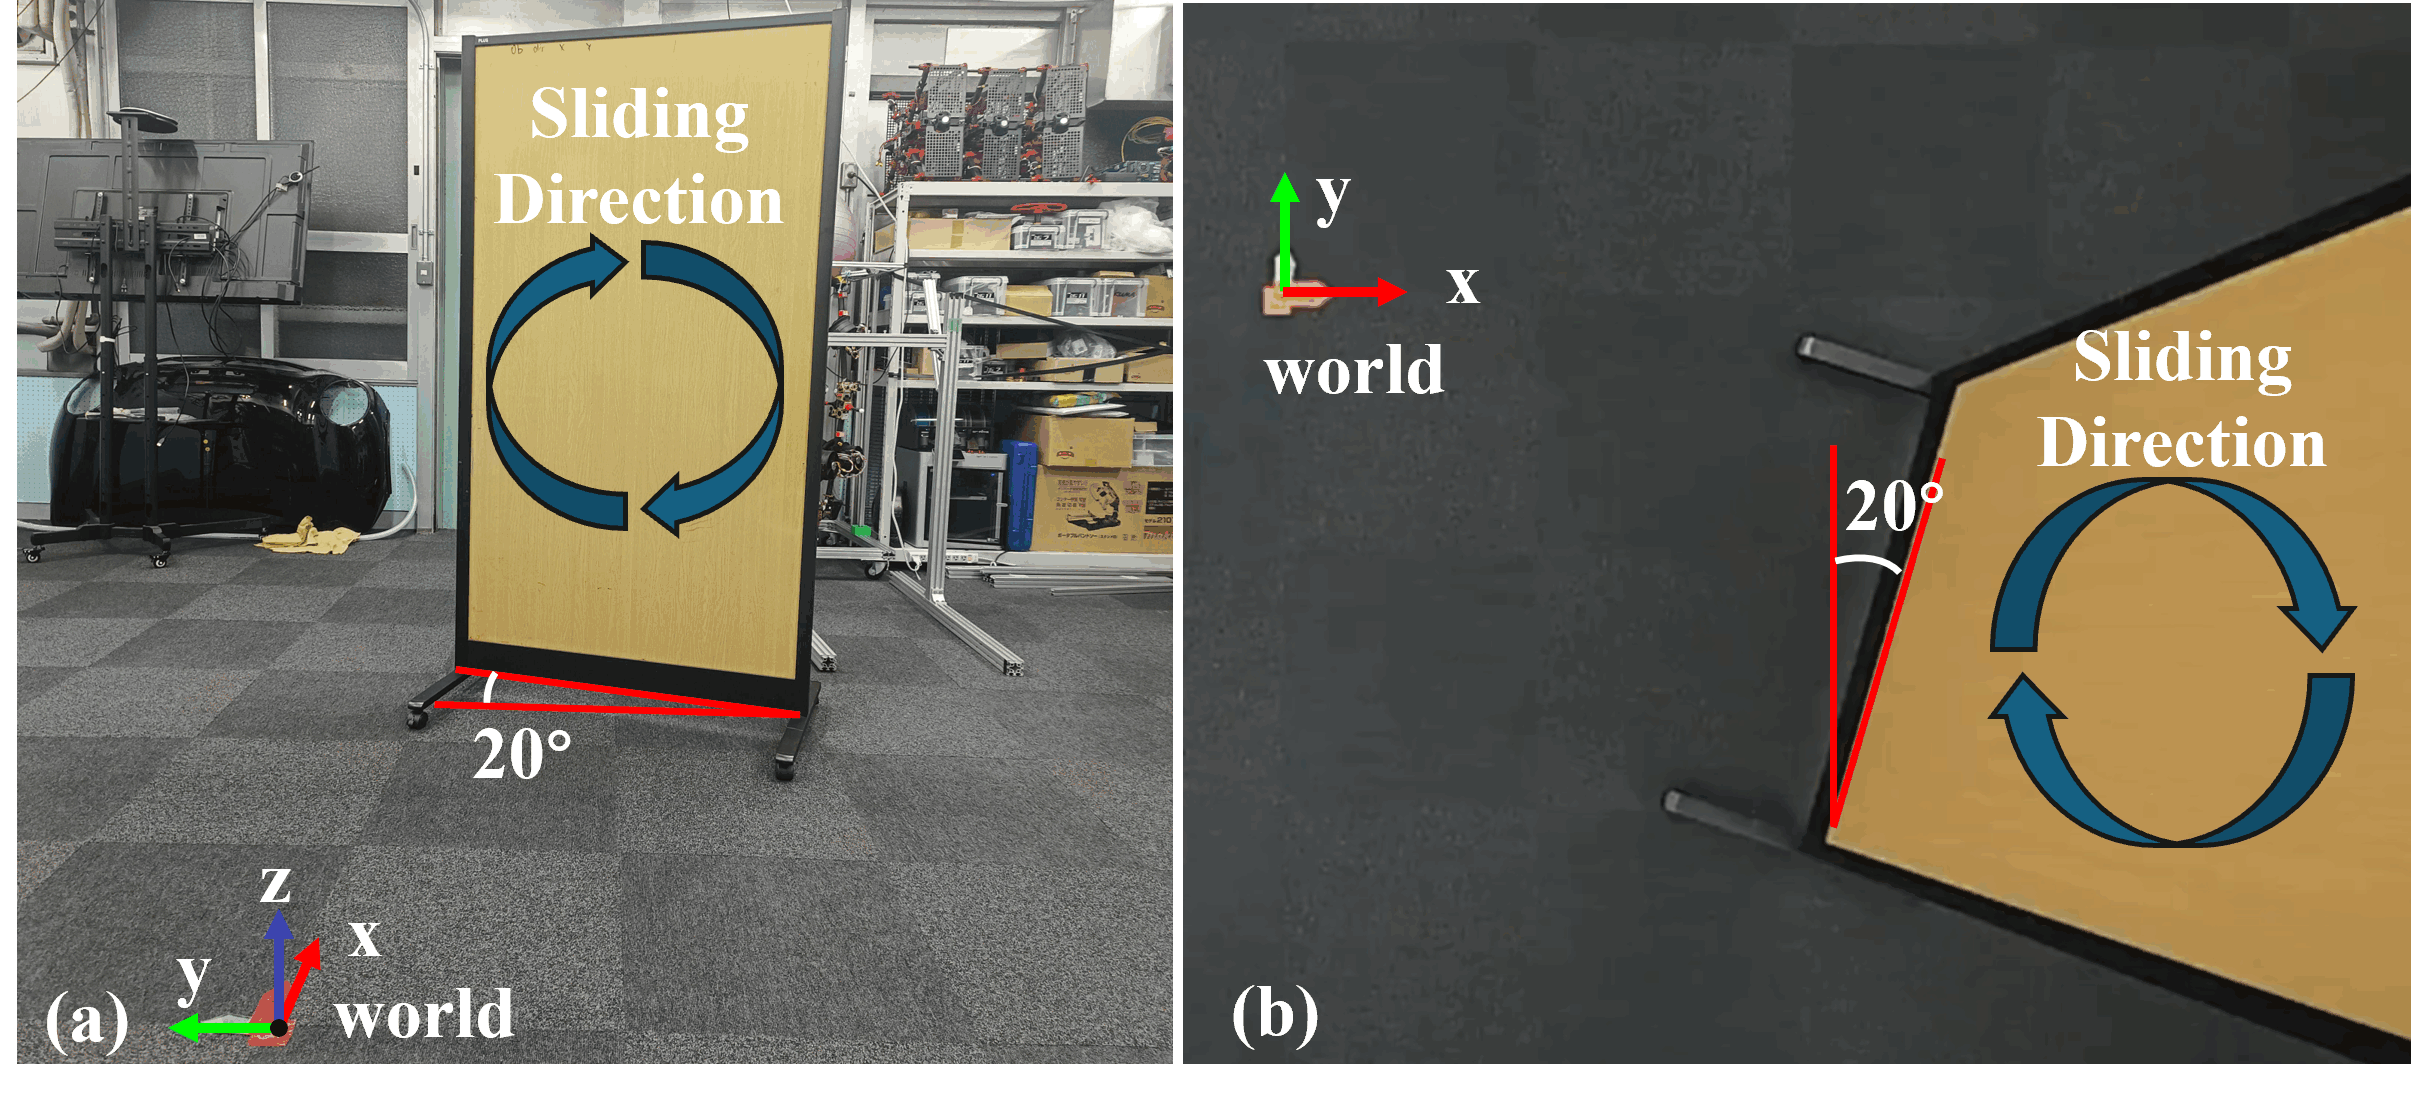
\includegraphics[trim={0cm 1cm 0cm 0cm}, clip, width=\linewidth]{figures/chapter6/exp_scene.png}
    \caption{Experiment scenario: an board with \textbf{known} position, and \textbf{unknown} sloped angle to the robot controller to mimic an unknown surface geometric variation. The world frame is marked on the figure. (A) Side view. (b) Top view.}
    \label{fig:exp_scene}
    \vspace{-5mm}
\end{figure}

During the experiment, the reference trajectory of the multi-link aerial robot was defined on a plane perpendicular to the $x$ axis. The robot was commanded to follow the predefined circular trajectory with a radius of $0.30\,\mathrm{m}$ and a period of $14\,\mathrm{s}$ within this plane. Due to the board's unknown inclination angle, the desired circular trajectory experienced approximately $0.15\,\mathrm{m}$ of variation along the $x$ axis during one cycle, introducing measurable geometry-induced deviations during contact. This geometric variation was not incorporated into the reference trajectory generation or controller design. Therefore, the robot was required to adapt to this geometric variation online during contact.

To evaluate performance, we conducted comparative experiments between the proposed hybrid controller and a manually tuned PID baseline. The PID gains were selected to provide the best stable tracking performance in free flight and were kept identical to the proportional and derivative gains used in the impedance controller. In the hybrid controller, impedance control was applied along the $y$ and $z$ axes to improve sliding resilience, while admittance control was applied along the $x$ axis to enable adaptive surface interaction. Note that each controller is executed independently along its respective axis. To demonstrate the necessity of combining impedance control and admittance control, we additionally performed experiments using only impedance control (without admittance-based joint adaptation) and only admittance control (where the CoG state was regulated solely by PID).


\begin{figure}[!htbp]
    \centering
    % \parbox{3in}
    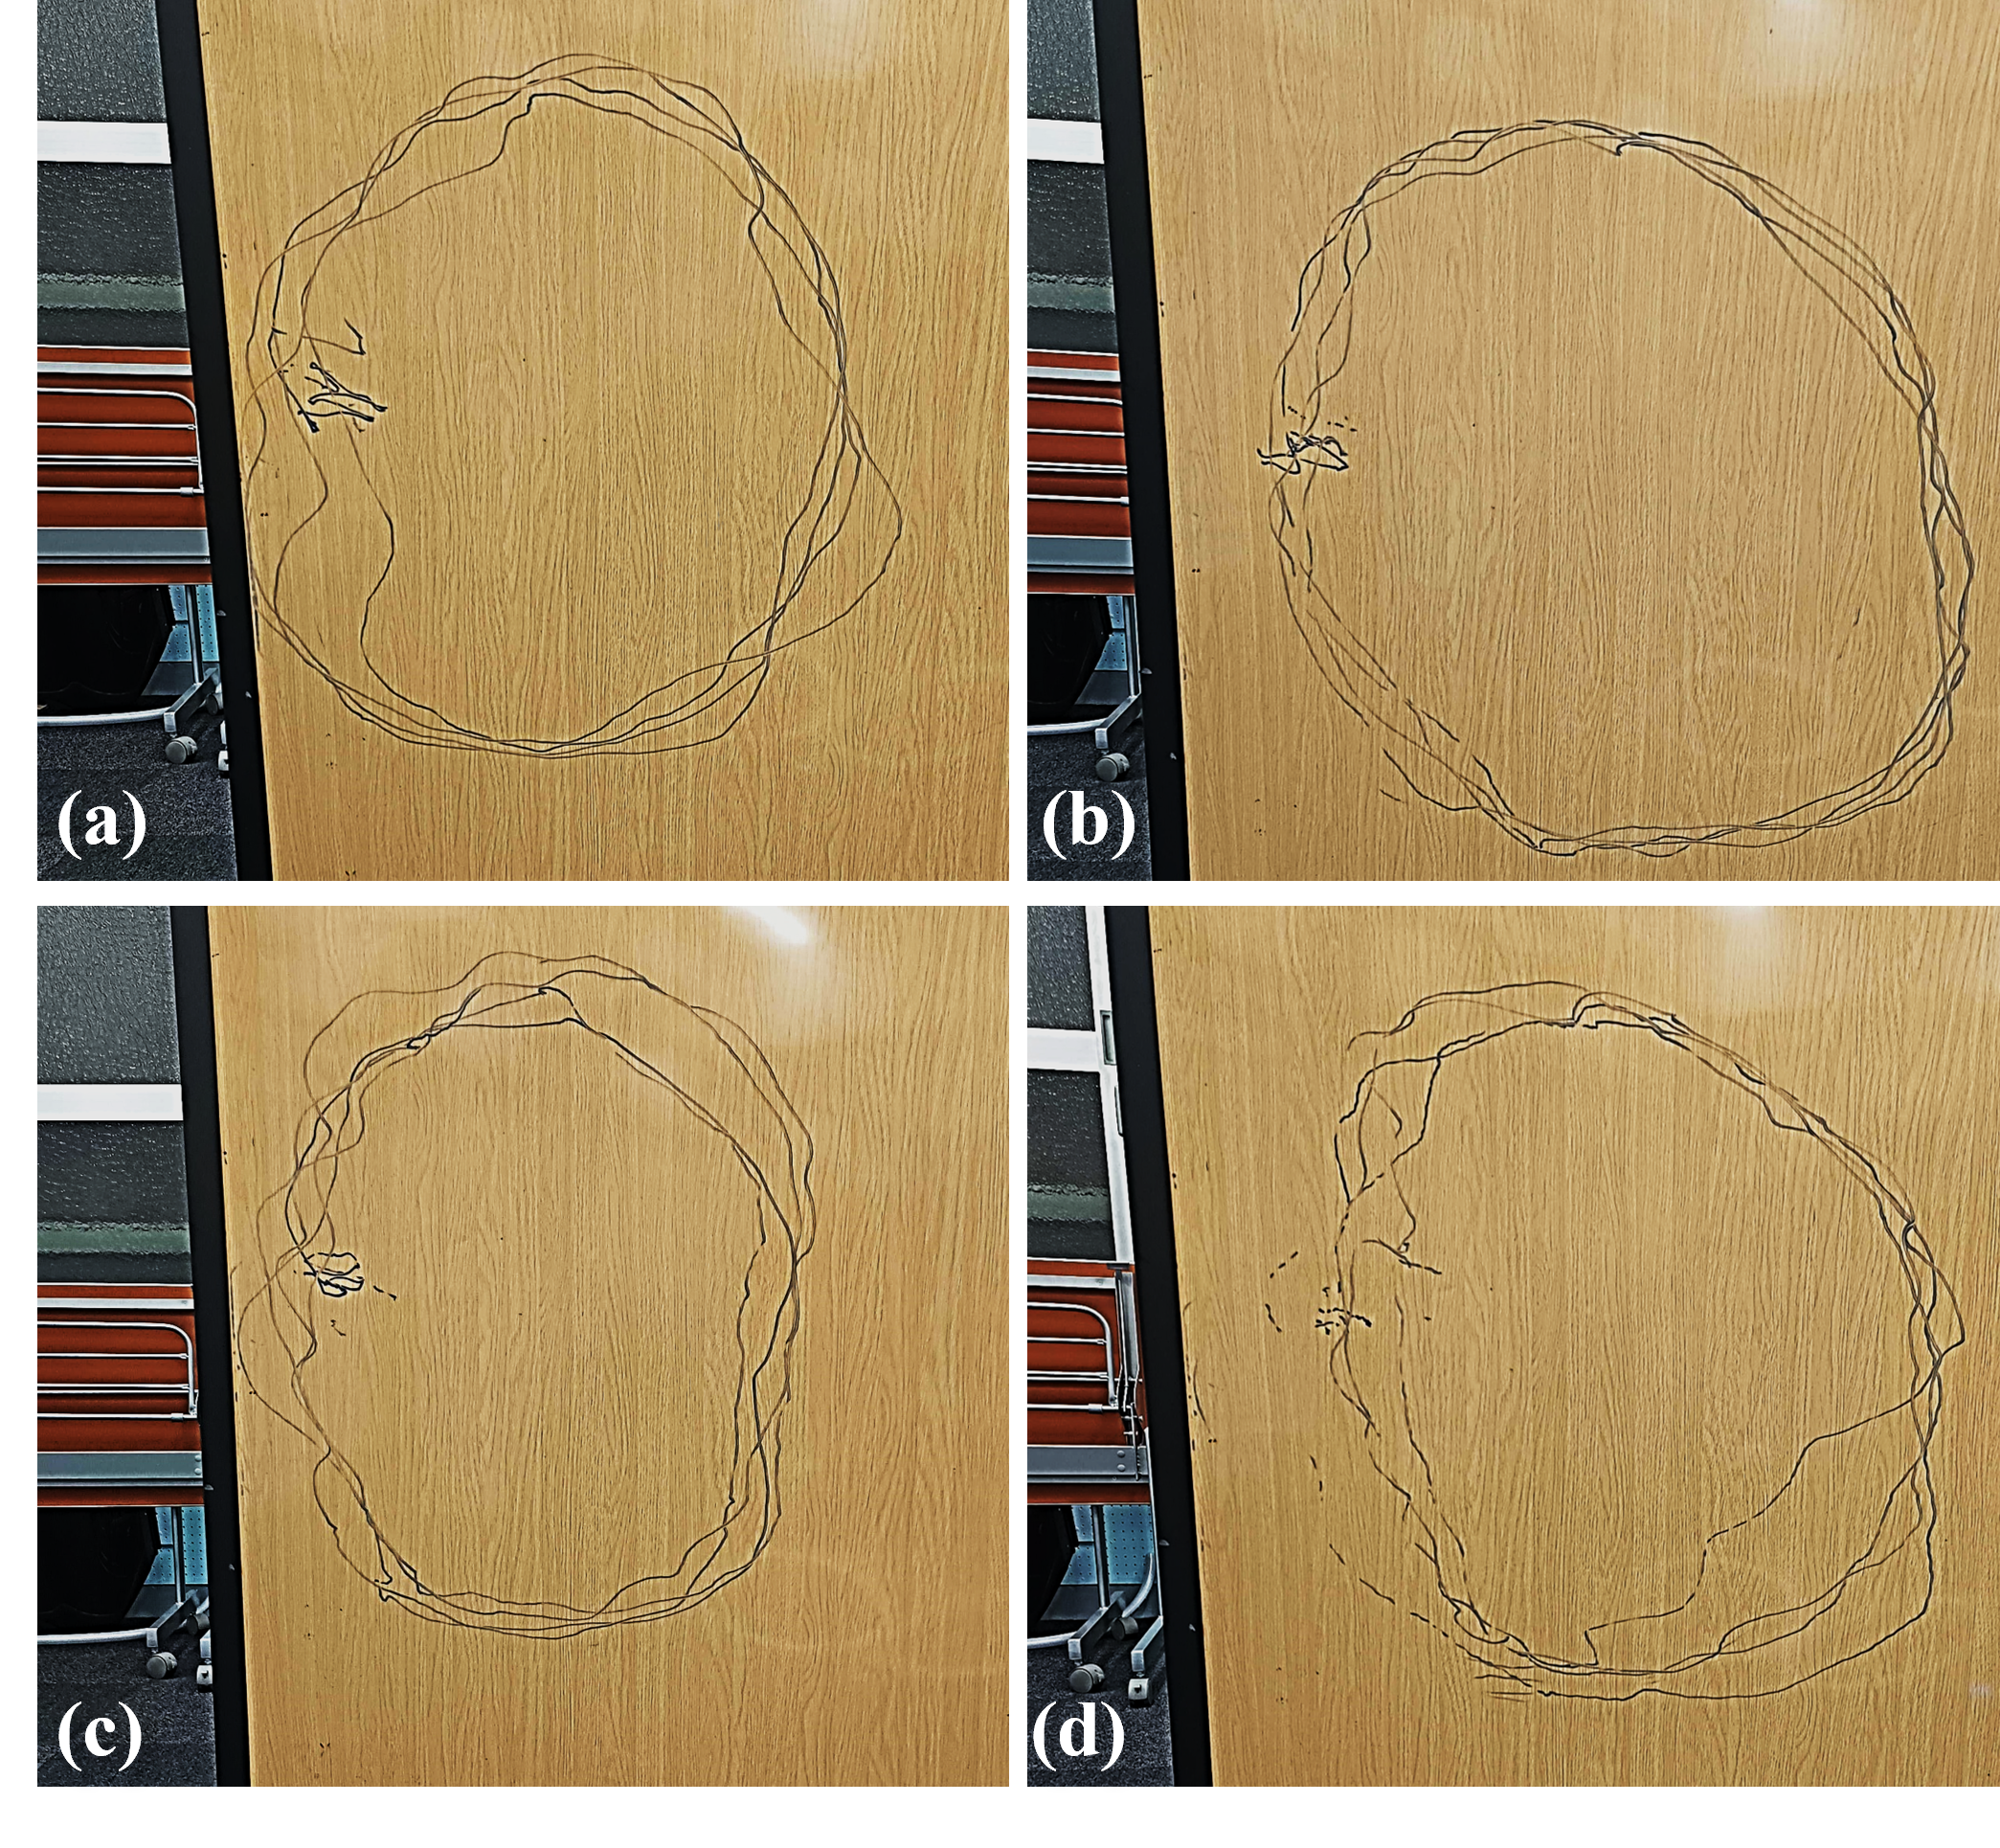
\includegraphics[trim={0cm 0cm 0cm 0cm}, clip, width=\linewidth]{figures/chapter6/experiment_trajectory.png}
    \caption{Tracking trajectory on the board. (a) PID controller. (b) Only impedance controller. (c) Only admittance controller. (d) Hybrid impedance-admittance controller.}
    \label{fig:impedance_result}
\end{figure}

\begin{figure}[!htbp]
    \centerline{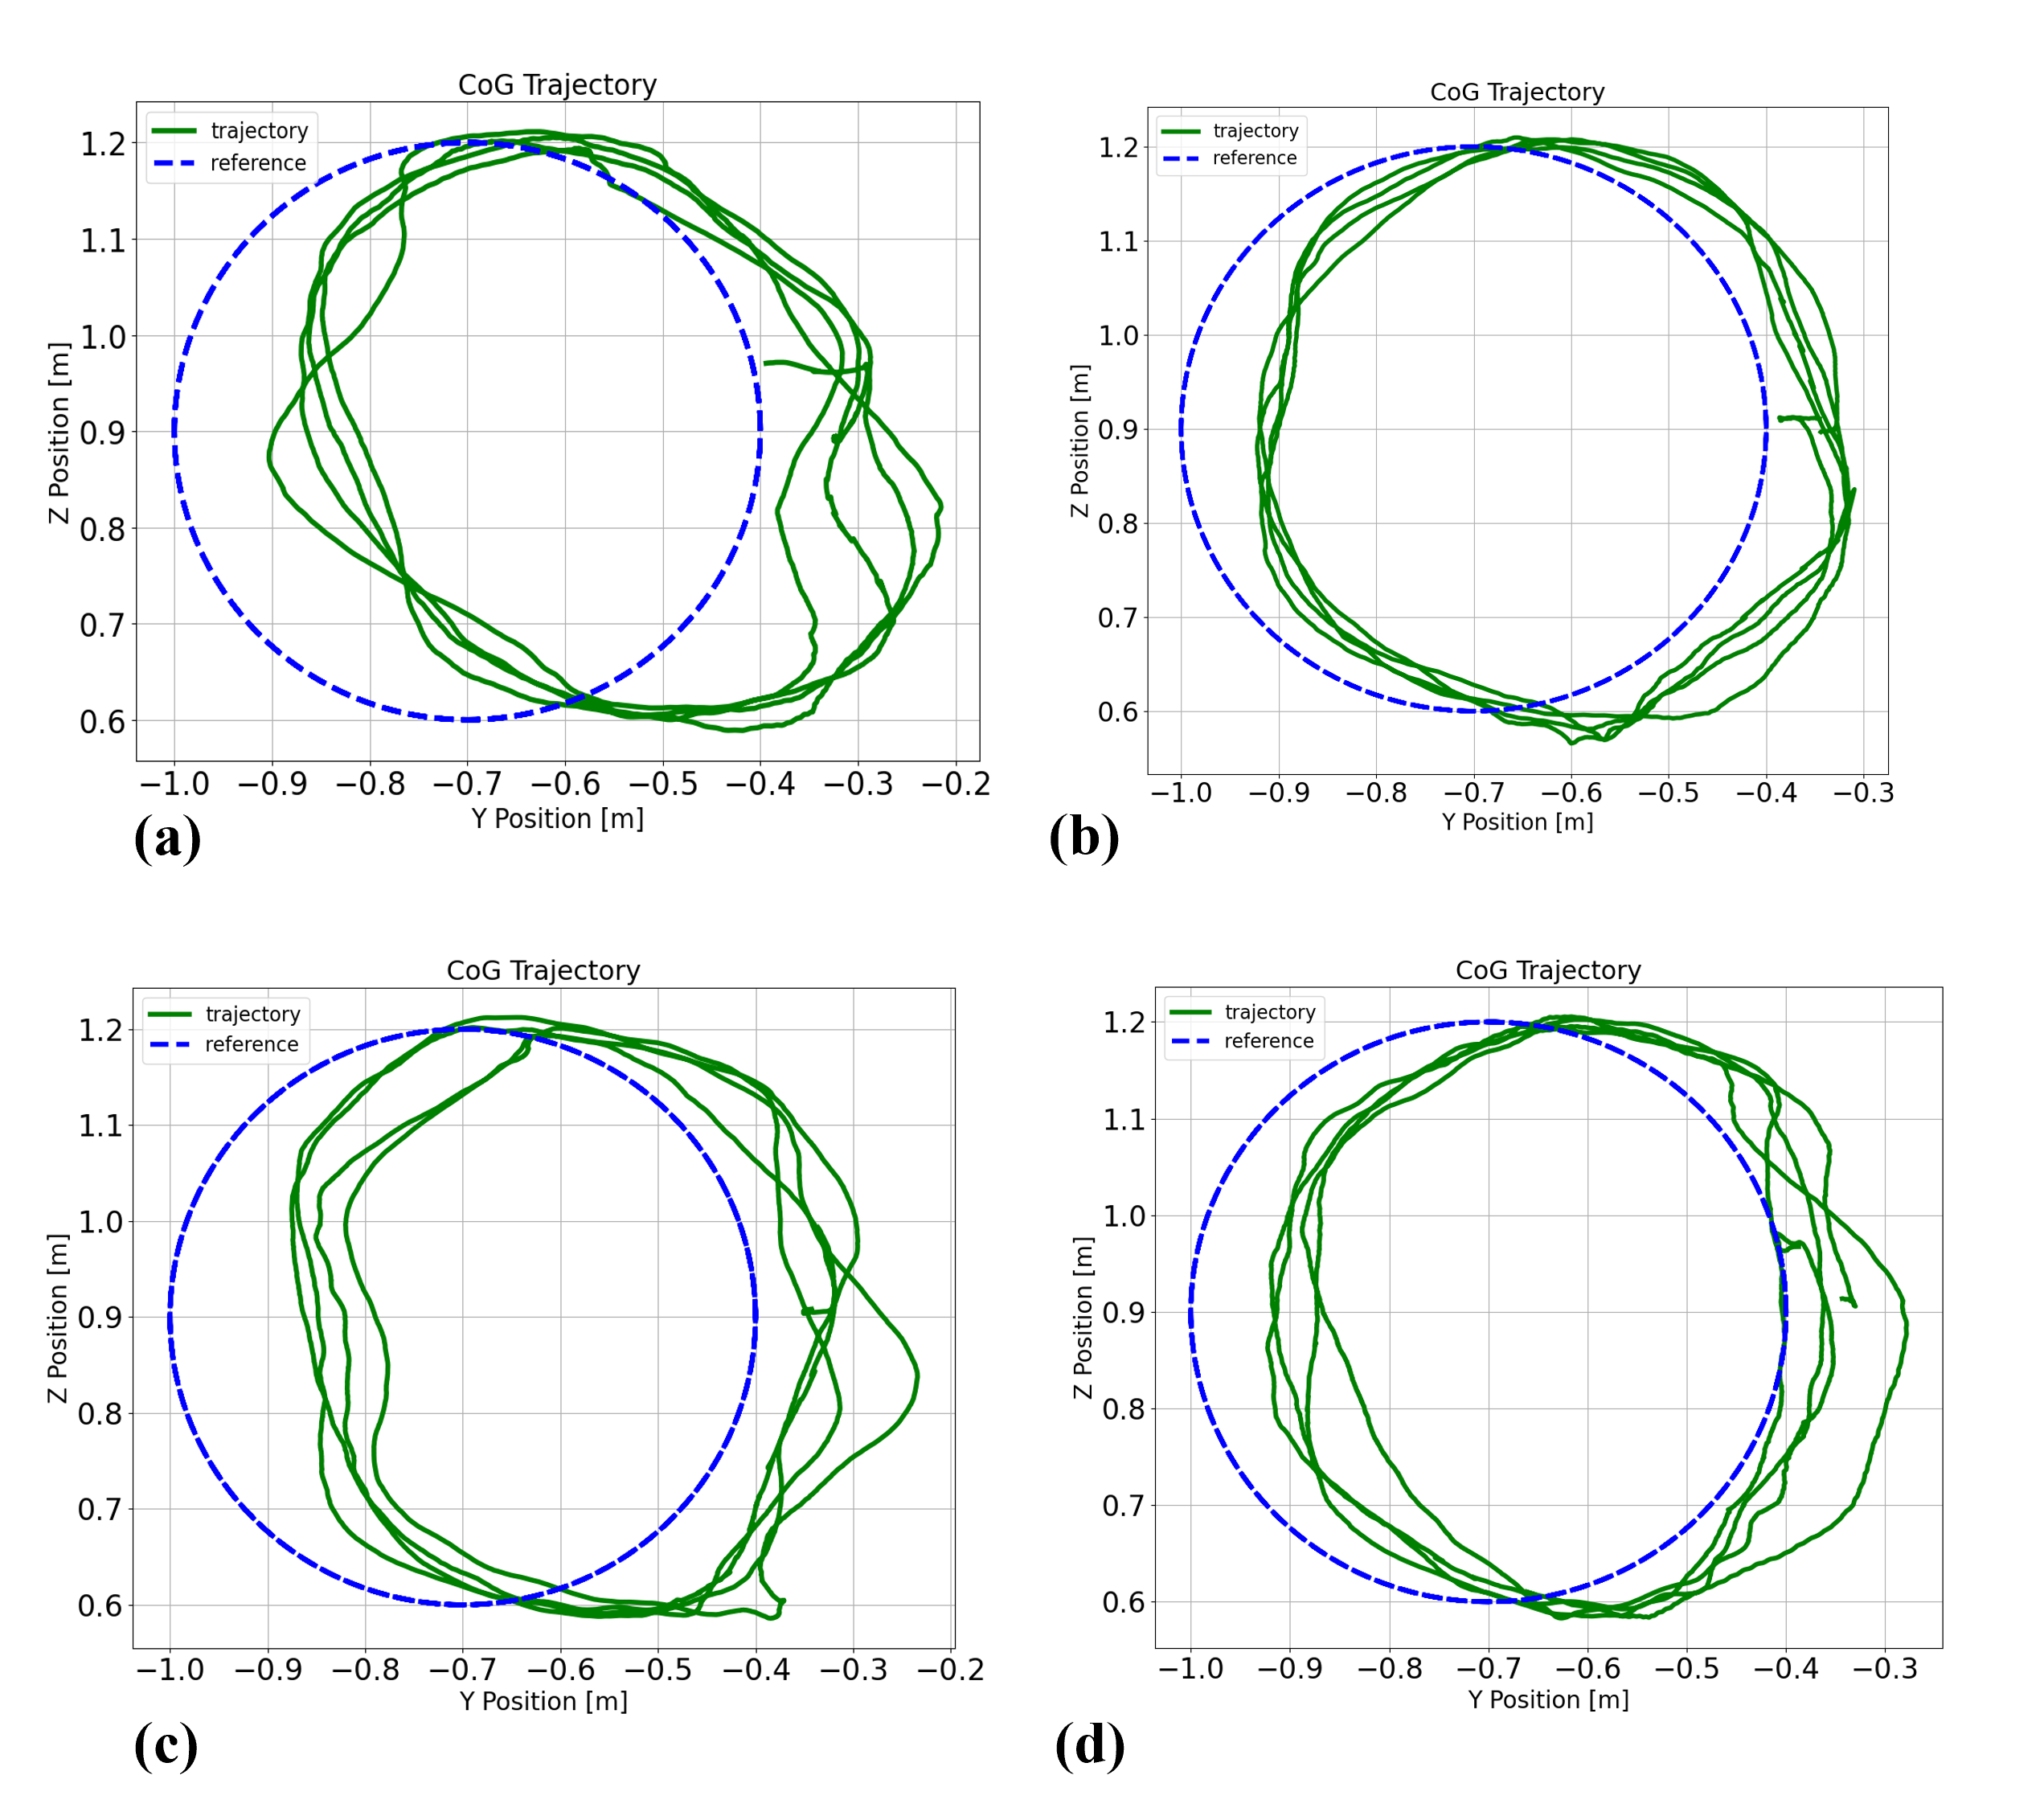
\includegraphics[trim=0 0 0 0,clip,width=\linewidth]
    {figures/chapter6/trajectory_plot.png}}
    \caption{Circle trajectory tracking result of the CoG under four controllers. (a) PID controller. (b) Only impedance controller. (c) Only admittance controller. (d) Hybrid impedance-admittance controller.}
    \label{fig:trajectory_plot}
\end{figure}
Following this setup, four sets of experiments were performed. Fig.~\ref{fig:impedance_result} shows the final trajectories drawn on the board, and Fig.~\ref{fig:impedance_result} shows the reference and real trajectory data. Overall, the only impedance control produced a trajectory closest to the desired circle, while the hybrid controller showed a nearly circular path. In contrast, only admittance control and PID control resulted in noticeably smaller and more distorted trajectories. Fig.~\ref{fig:impedance_result} shows the RASE of the trajectory, we can also find that the impedance performs better in the experiments.

Fig.~\ref{fig:admittance_exp} further illustrates how the multi-link aerial robot deformed to accommodate geometric variations during contact under hybrid controller by taking the spotphoto. We can see that in the leftside where the geometry variation is small, the structure become long to keep contact with the broad. On the other hand, in the right side where the geometry variation is large, the structure shrink to adapt to the variation to reduce the CoG displacement in order to improve stability.


\begin{figure}[!htbp]
    \centerline{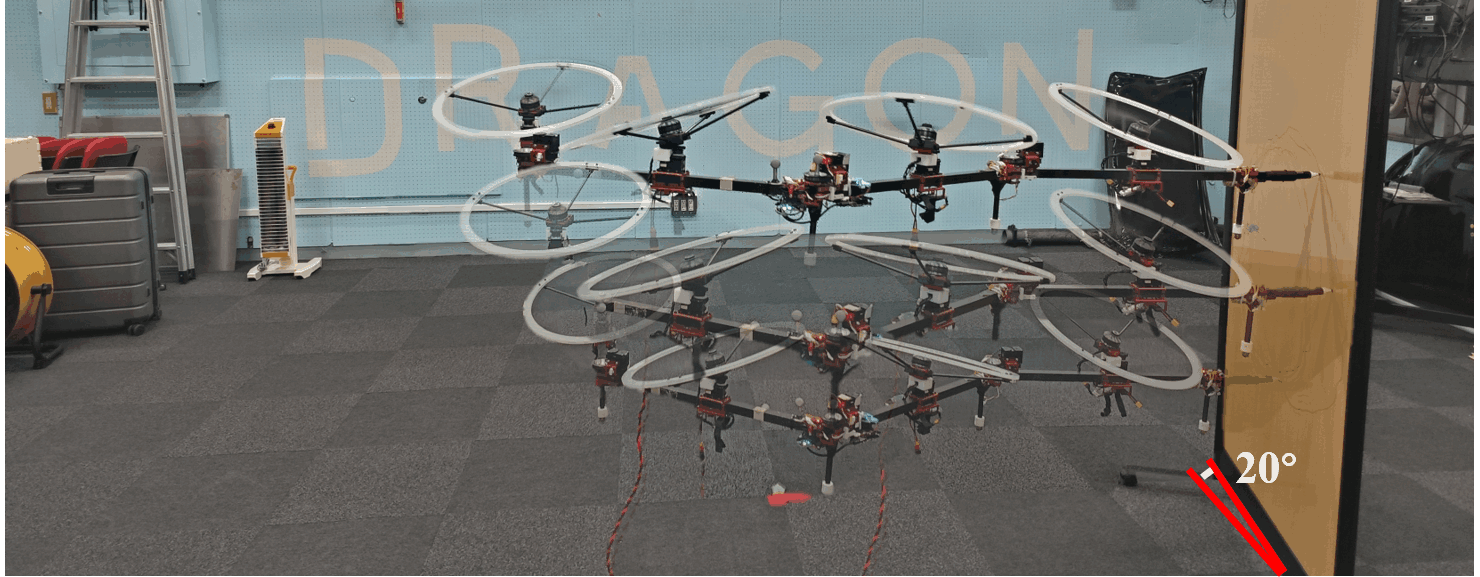
\includegraphics[trim=0 0 0 0,clip,width=\linewidth]
    {figures/chapter6/admittance_exp.png}}
    \caption{The hybrid controller enabled the multi-link aerial robot to deform appropriately when encountering surface geometric variation. (a) Top view. (b) Front view.}
    \label{fig:admittance_exp}
\end{figure}


\subsection{Compare on Impedance-related direction}

Fig.~\ref{fig:impedance_plot} presents the CoG trajectories together with the reference path under the four controllers. Note that during the sliding task, the $y$ and $z$ axes corresponded to the sliding directions, where friction-induced disturbances were dominant. Although Fig.~\ref{fig:impedance_plot} illustrates the overall trajectories of the four controllers, their performance differences become more evident in the tracking error distributions shown in Fig.~\ref{fig:impedance_box}. The figure shows the distributions of tracking errors of the CoG in the $y$ and $z$ axes. In particular, the median $y$ axis errors were approximately $0.134\,\mathrm{m}$ for PID control, $0.079\,\mathrm{m}$ for only impedance control, $0.105\,\mathrm{m}$ for only admittance control, and $0.083\,\mathrm{m}$ for the hybrid controller. These results indicate that impedance-based methods provided more stable tracking performance than the conventional PID controller when sliding under friction.

This part of the experiments shows that along the sliding directions, impedance control provided a resilient response to frictional disturbances, enabling more accurate sliding without requiring explicit friction values while still approximately following the desired trajectory.


\begin{figure}[!htbp]
    \centerline{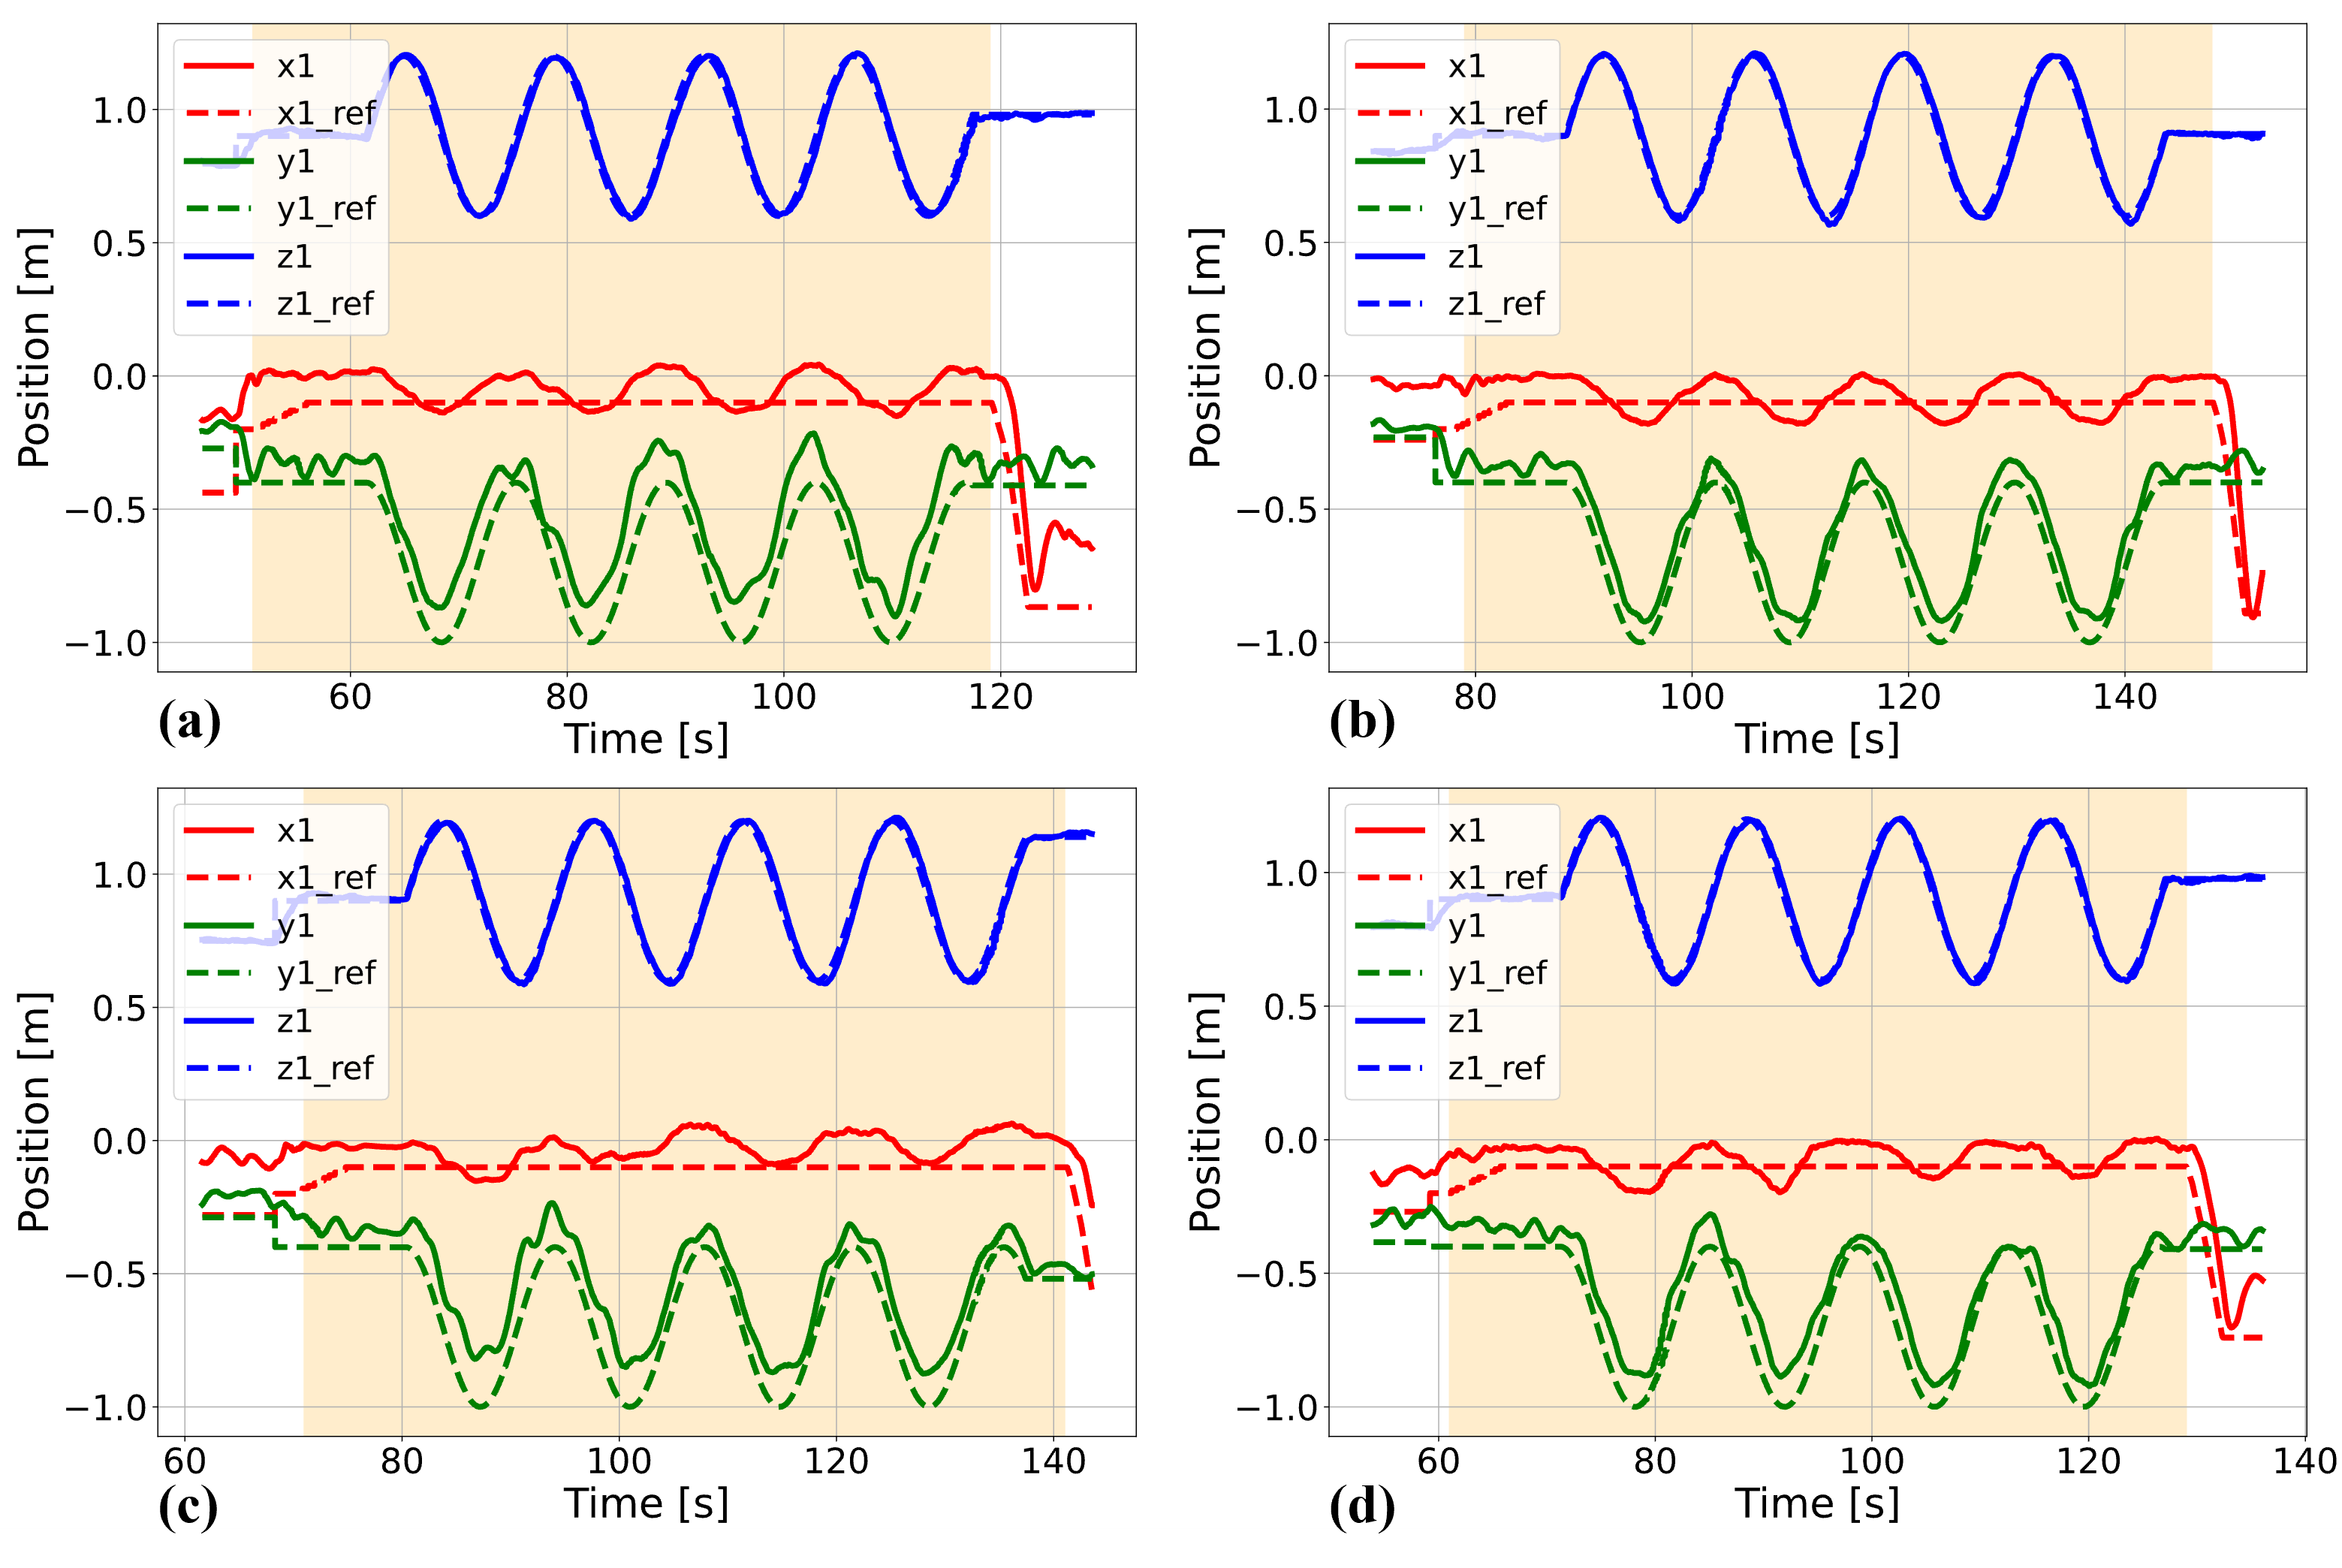
\includegraphics[trim=0 0 0 0,clip,width=\linewidth]
    {figures/chapter6/imp_plot.png}}
    \caption{Circle trajectory tracking result of the CoG under four controllers. (a) PID controller. (b) Only impedance controller. (c) Only admittance controller. (d) Hybrid impedance-admittance controller. The yellow region denotes the contacting period. }
    \label{fig:impedance_plot}
\end{figure}



\begin{figure}[!htbp]
    \centerline{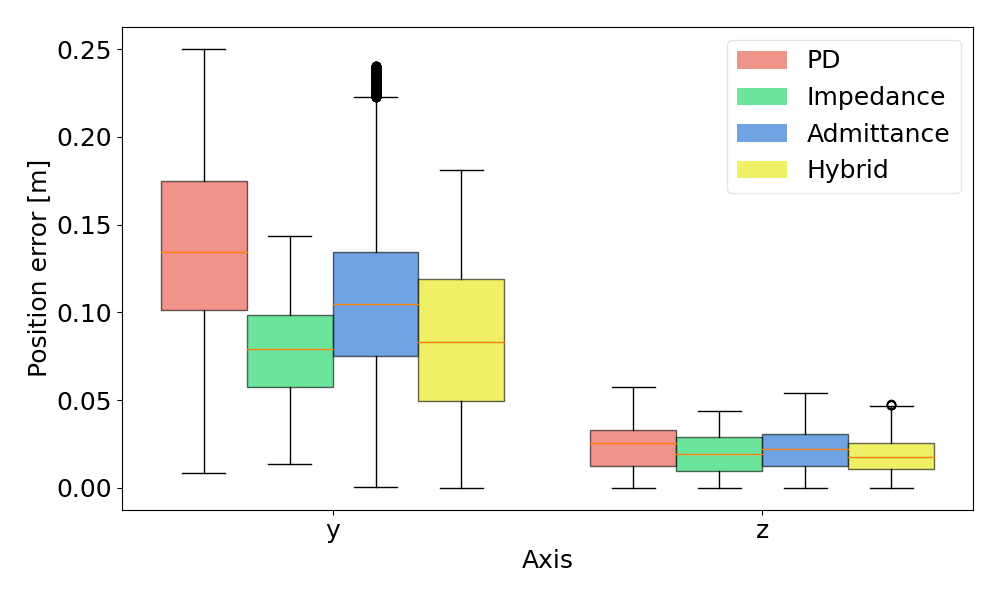
\includegraphics[trim=0 0 0 0,clip,width=\linewidth]
    {figures/chapter6/box_position.png}}
    \caption{Box plots of position errors along the sliding directions (the $y$ and $z$ axes) under the four controllers during the contact period.}
    \label{fig:impedance_box}
\end{figure}


\subsection{Compare on Admittance-related direction}

Fig.~\ref{fig:admittance_plot} shows the CoG displacement and external force along the $x$ axis. As further quantified in Fig.~\ref{fig:admittance_box}, the PID and only impedance controllers produced similar CoG displacements ($0.133\,\mathrm{m}$ and $0.137\,\mathrm{m}$), both largely reflecting the board's deformation. In contrast, the admittance and hybrid controllers reduced the CoG displacement to $0.088\,\mathrm{m}$ and $0.084\,\mathrm{m}$, demonstrating their effectiveness in mitigating geometric variation effects.

Fig.~\ref{fig:admittance_box} also shows that the median external forces on the CoG were approximately $-1.190\,\mathrm{N}$ for the PID controller, $-0.453\,\mathrm{N}$ for the only impedance controller, $-0.712\,\mathrm{N}$ for the only admittance controller, and $-0.328\,\mathrm{N}$ for the hybrid controller. The hybrid controller achieved the smallest median external force. In addition, the admittance and hybrid controllers exhibited relatively narrower force distributions than the PID controller, indicating more stable and adaptive interactions with the uncertain surface.

These improvements demonstrate that the admittance controller enables the robot to adjust its configuration in response to surface geometric variations, thereby reducing the influence of geometric variations on the CoG and improving the contact force behavior.

\begin{figure}[!htbp]
    \centerline{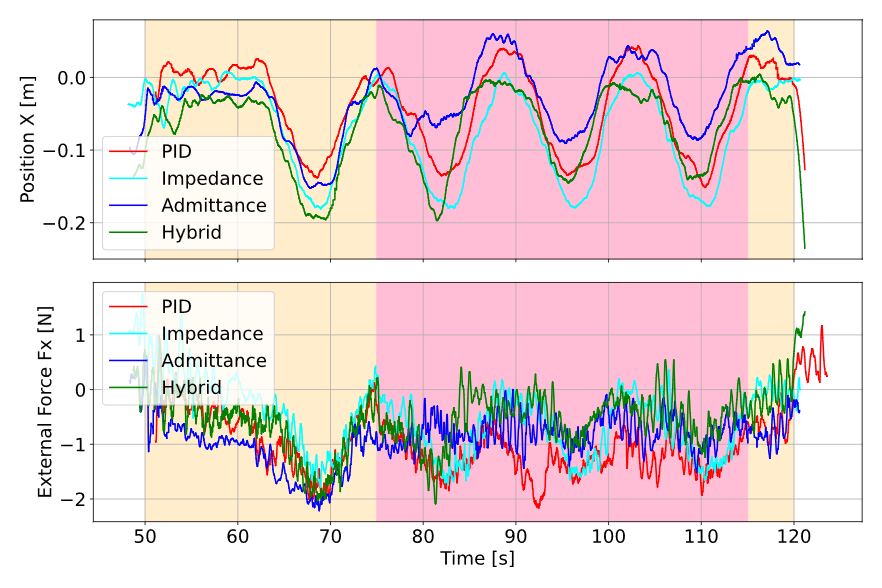
\includegraphics[trim=0 0 0 0,clip,width=\linewidth]{figures/chapter6/admittance_plot.png}}
    \caption{Plot of position variation and external force on the CoG in the $x$ axis. The yellow region denotes the contact period, and the pink region indicates the interval during which the admittance controller actively adjusts the configuration.}
    \label{fig:admittance_plot}
\end{figure}

\begin{figure}[!htbp]
    \centerline{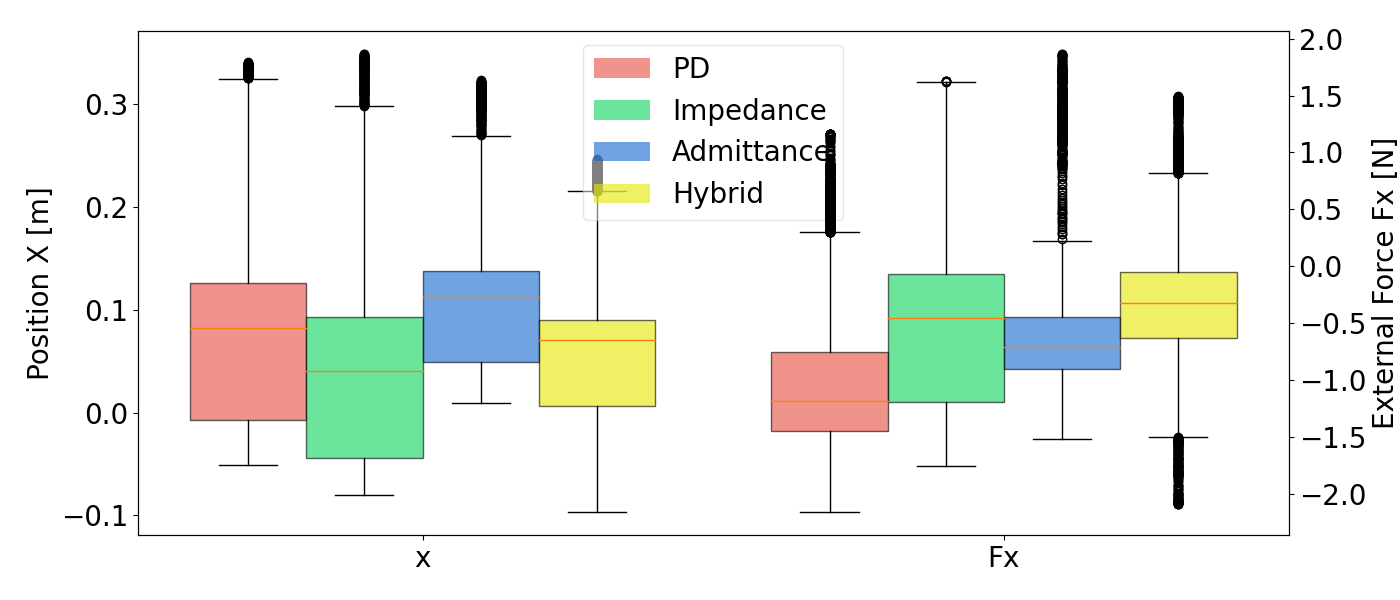
\includegraphics[trim=0 0 0 0,clip,width=\linewidth]
    {figures/chapter6/box_force.png}}
    \caption{Box plots of CoG position and CoG external force along the contact direction ($x$ axis) for the four controllers during the period when the admittance controller was active.}
    \label{fig:admittance_box}
\end{figure}

\subsection{Compare on All Directions}
Table shows the data of the four controllers. The hybrid controller get the best performance.
Table.~\ref{tb:hybrid} shows the CoG displacement error compares with the tracking error in y axis. We can see that in each, the hybrid controller performs as good as the only impedance controller or the only admittance controller. However, if we consider all the factor, the hybrid controller can achieve small CoG movement,simutenally. Therefore, the hybrid

\begin{table}[H]
    \centering
    \caption{Parameters of free flight.}
    \label{tb:hybrid}
    \begin{tabular}{|l|c|c|c|c|}
        \hline
        & PD & Impedance & Admittance & Hybrid \\
        \hline
        Y position error & $0.134\mathrm{m}$ & \textcolor{red}{$0.079\mathrm{m}$} &$0.105\mathrm{m}$ & \textcolor{brown}{$0.083\mathrm{m}$} \\
        Z position error & $0.026\mathrm{m}$ & \textcolor{brown}{$0.021\mathrm{m}$} & $0.024\mathrm{m}$ & \textcolor{red}{$0.020\mathrm{m}$} \\
        X displacement & $0.133\mathrm{m}$ & $0.137\mathrm{m}$ & \textcolor{brown}{$0.088\mathrm{m}$} & \textcolor{red}{$0.084\mathrm{m}$} \\
        X external & $-1.190\mathrm{N}$ & \textcolor{brown}{$-0.453\mathrm{N}$} & $-0.712\mathrm{N}$ & \textcolor{red}{$-0.328\mathrm{N}$} \\
        \hline
    \end{tabular}
\end{table}

\subsection{Section summary}
The experiment highlights the complementary roles of the two strategies: impedance control improves sliding smoothness and reduces tracking error, whereas admittance control enhances adaptive interaction by decreasing both displacement and contact forces. Since neither only impedance controller nor only admittance controller alone can achieve both behaviors, the hybrid controller yields smaller trajectory deviations, reduced unintended CoG drift, and lower interaction forces compared with the baseline PID controller, confirming its effectiveness for compliant contact-rich tasks.


%%%%%%%%%%%%%%%%%%%%%%%%%%%%%%%%%%%%%%%%%%%%%%%%%%%%%%%%%%%%%%%%%%%%%%%%%%%%%%%%
\section{Extension Experiment on DRAGON}
\subsection{Experimental Setup}
Experiments are conducted using the multi-link aerial robot shown in Fig.~\ref{fig:robot}. The platform is equipped with an UP-Board single-board computer featuring an Intel Atom x5-Z8350 CPU, and the Robot Operating System (ROS) is utilized for communication. A motion capture system provides the full state of the robot throughout the experiments. A marker pen is attached to link 4 as shown in Fig.~\ref{fig:admittance control} and serves as the end-effector for maintaining contact with the environment.

We also test the sliding expeirment by DRAGON. The basic experiment setting is basically similar to Hydrus Xi's case. The parameters are shown in Table. Note that DRAGON is a 3D deformable mutli-link aerial robot, which has 6 joints to realize full DOF. In this expeirment, we only simply test whether the hybrid controller used in Hydrus Xi can also be used in DRAGON. Therefore, only 3 $Yaw$ joints were used.

% The actual experimental parameters are as follows. The estimator translation and rotation gain matrices are given by $\boldsymbol{K}_{ti}=diag(3.0, 3.0, 3.0)$ and $\boldsymbol{K}_{ri}=diag(1.0, 1.0, 1.0)$. We treat $\boldsymbol{M}_d/m$ and $\boldsymbol{I}_d\boldsymbol{I}^{-1}$ as entities. Their values are set to $\boldsymbol{M}_d/m=diag(1.0, 3.0, 1.0)$, $\boldsymbol{I}_d\boldsymbol{I}^{-1}=diag(10.0, 10.0, 5.0)$. By choosing these values greater than $1$, the impedance controller exhibits more resilient behavior against environmental disturbances due to the increased designed stiffness. The normalized linear stiffness and rotational stiffness are given by $\tilde{\boldsymbol{K}}_{td} = diag(2.5, 2.5, 1.5)$, $\tilde{\boldsymbol{K}}_{rd} = diag(40.0, 40.0, 10.0)$. The normalized linear and rotational damping terms are not directly specified. Instead, we define the linear damping ratio $\boldsymbol{Z}_{td}=diag(0.6, 0.6, 0.7)$ and the rotational damping ratio $\boldsymbol{Z}_{rd}=diag(1.1, 1.1, 0.8)$, and compute the corresponding normalized damping matrices as follows:
% \begin{subequations}
% \label{eq:damping rate}
% \begin{align}
% \tilde{\boldsymbol{C}}_{td}&=2\boldsymbol{Z}_{td}\tilde{\boldsymbol{K}}^{\frac{1}{2}}_{td}, \\[2pt]
% \tilde{\boldsymbol{C}}_{rd}&=2\boldsymbol{Z}_{rd}\tilde{\boldsymbol{K}}^{\frac{1}{2}}_{rd}.
% \end{align}
% \end{subequations}
% The admittance mass, damping and stiffness are given by $m_a=40\,\mathrm{kg}$, $c_a=55\,\mathrm{N\cdot s/m}$ and $k_a=16\,\mathrm{N/m}$. The reference external force is given by $f_{ref,x} = 0$.
% \begin{figure}[t]
%      \centering
%     % \parbox{3in}
%     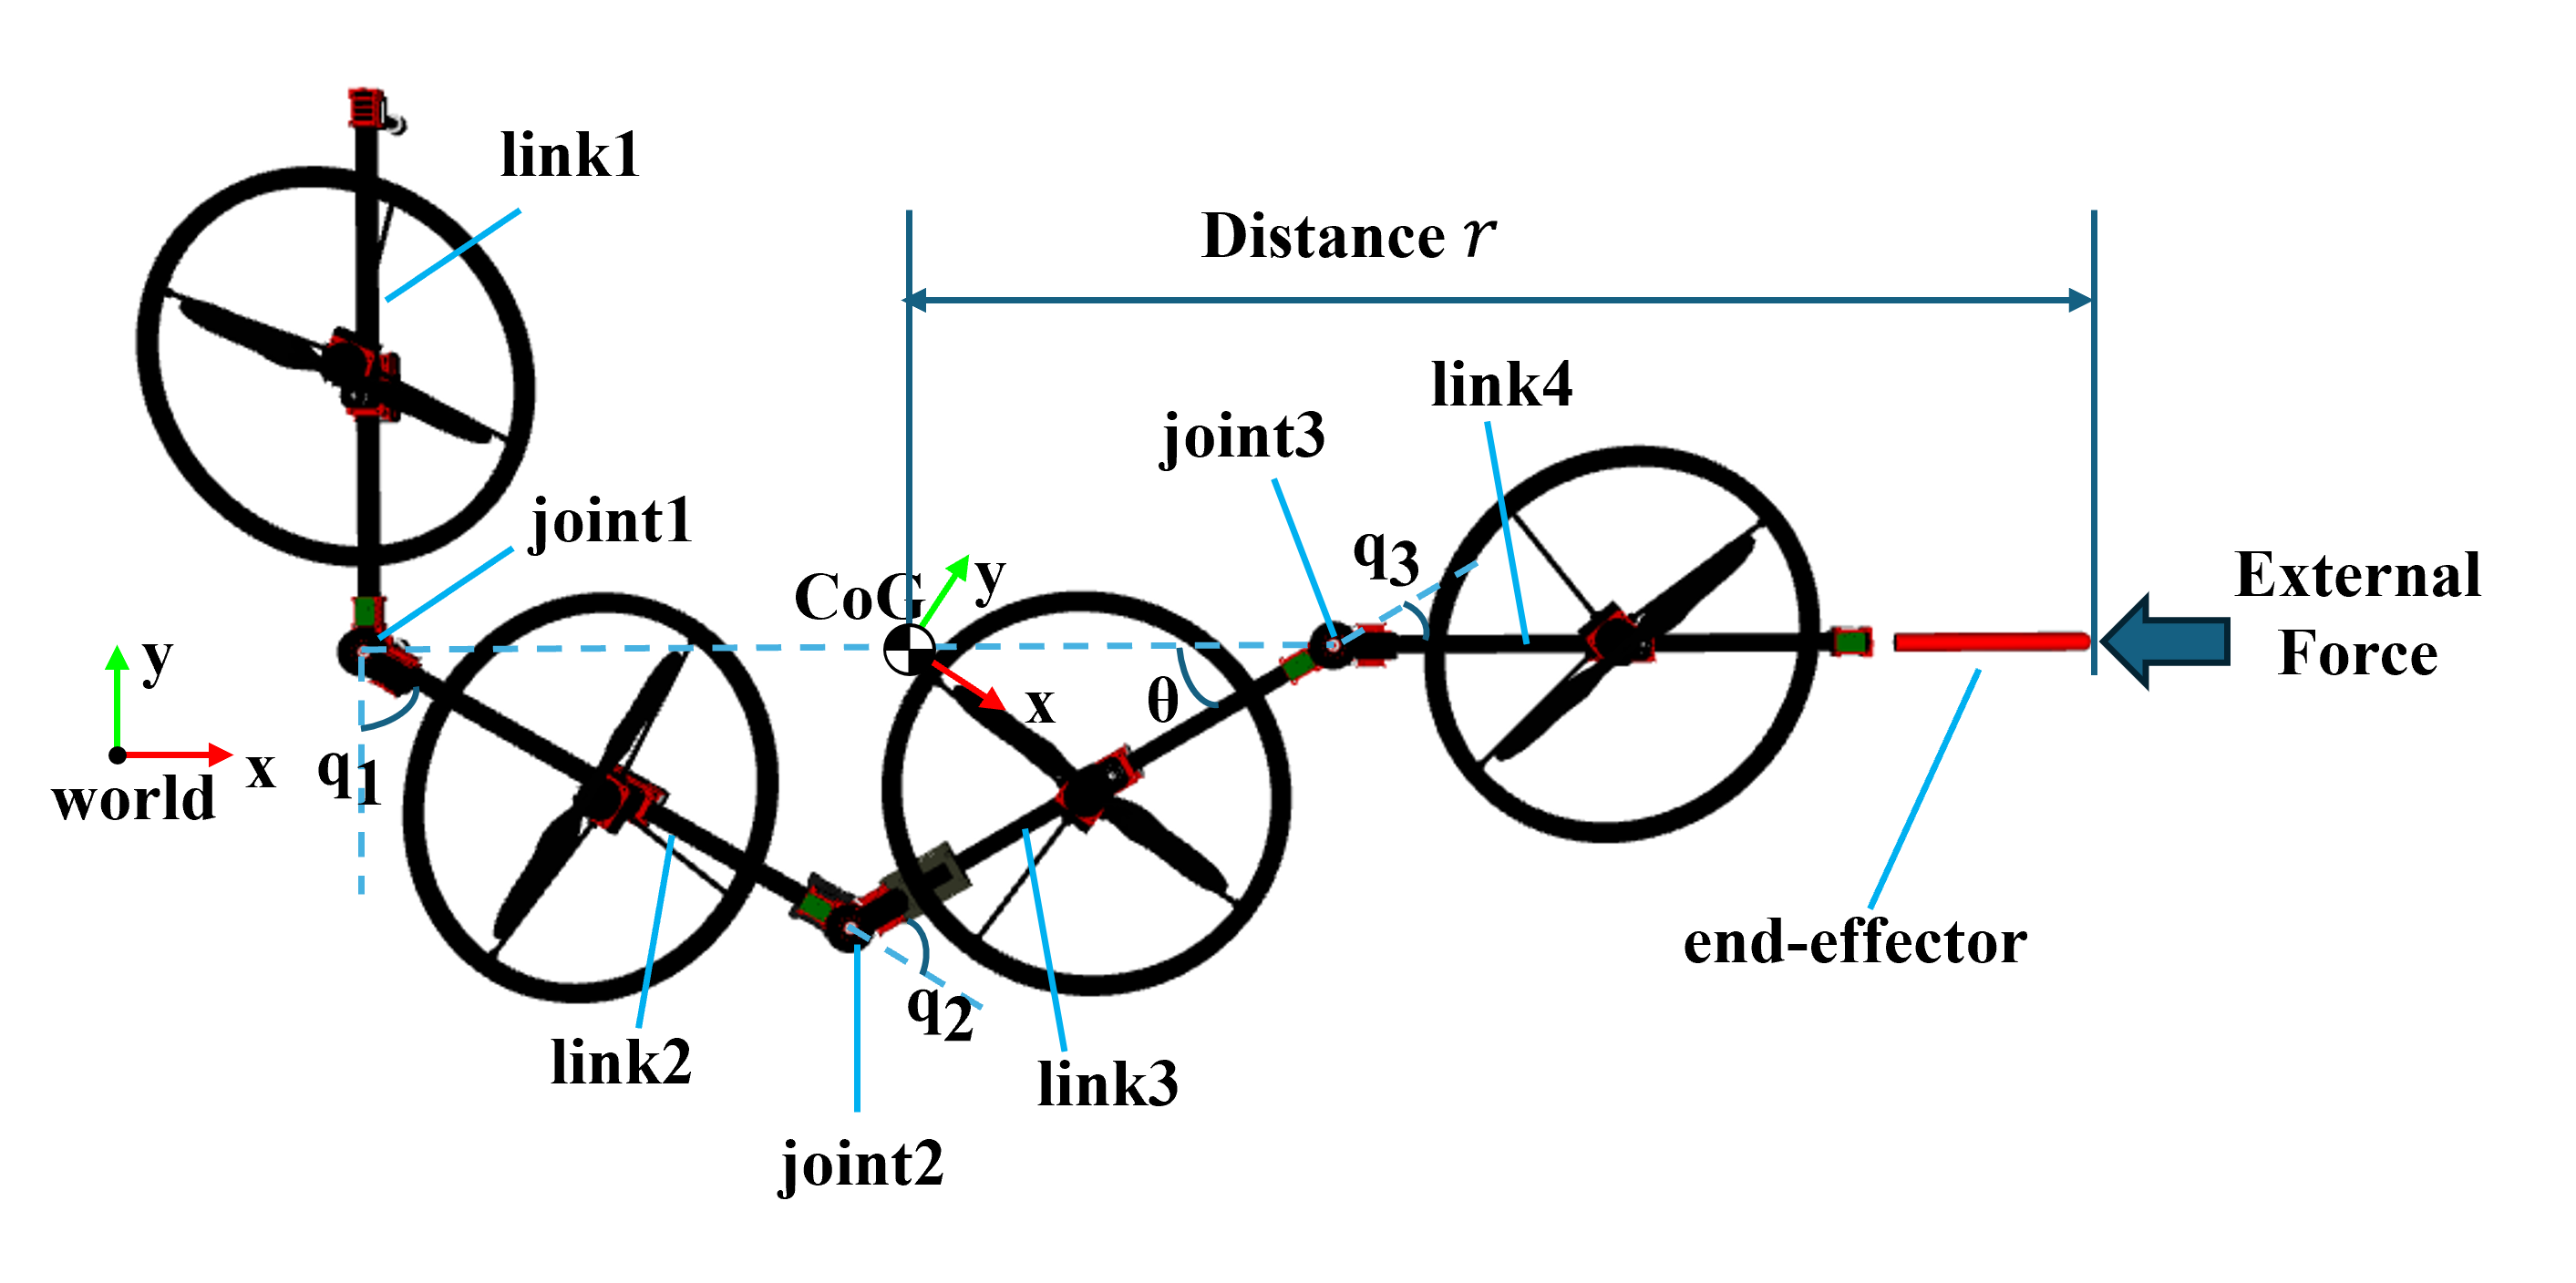
\includegraphics[trim={0cm 0.5cm 0cm 0cm}, clip, width=\linewidth]{figures/chapter5/hydrus.png}
%     \caption{The nominal surface-contact configuration of the multi-link aerial robot. The configuration angle $\theta = \pi /6$, and the joint angles $q_1$, $q_2$, $q_3$ are consequently $\pi /3, \pi /3,-\pi /6$, respectively.}
%     \label{fig:admittance control}
%     \vspace{-5mm}
% \end{figure}

As shown in Fig.~\ref{fig:admittance control}, the robot started from its nominal configuration. Throughout the experiment, a constant yaw angle was commanded, implemented by keeping link 4 aligned with the $x$ axis in order to reduce external torque applied on the CoG. 

During the experiment, the reference trajectory of the end effector of multi-link aerial robot was defined on a plane perpendicular to the $x$ axis. The robot was commanded to follow the predefined circular trajectory with a radius of $0.30\,\mathrm{m}$ and a period of $14\,\mathrm{s}$ within this plane. Due to the board's unknown inclination angle, the desired circular trajectory experienced approximately $0.15\,\mathrm{m}$ of variation along the $x$ axis during one cycle, introducing measurable geometry-induced deviations during contact. Meanwhile, the base link is set to stay at a static point in the frame of $\{W\}$. This geometric variation was not incorporated into the reference trajectory generation or controller design. Therefore, the robot was required to adapt to this geometric variation online during contact. It can be considered that the prior frame is requested to draw a circle in the board, and the secondary frame is requested to keep static in the air. 


As shown in Fig.~\ref{fig:dragon_experiment}. 

The original displacement in x is $0.115m$, whereas the real displacement is $0.065$. We can see that the distance in x is reduce $0.08m$.

\begin{figure}[!htbp]
    \centerline{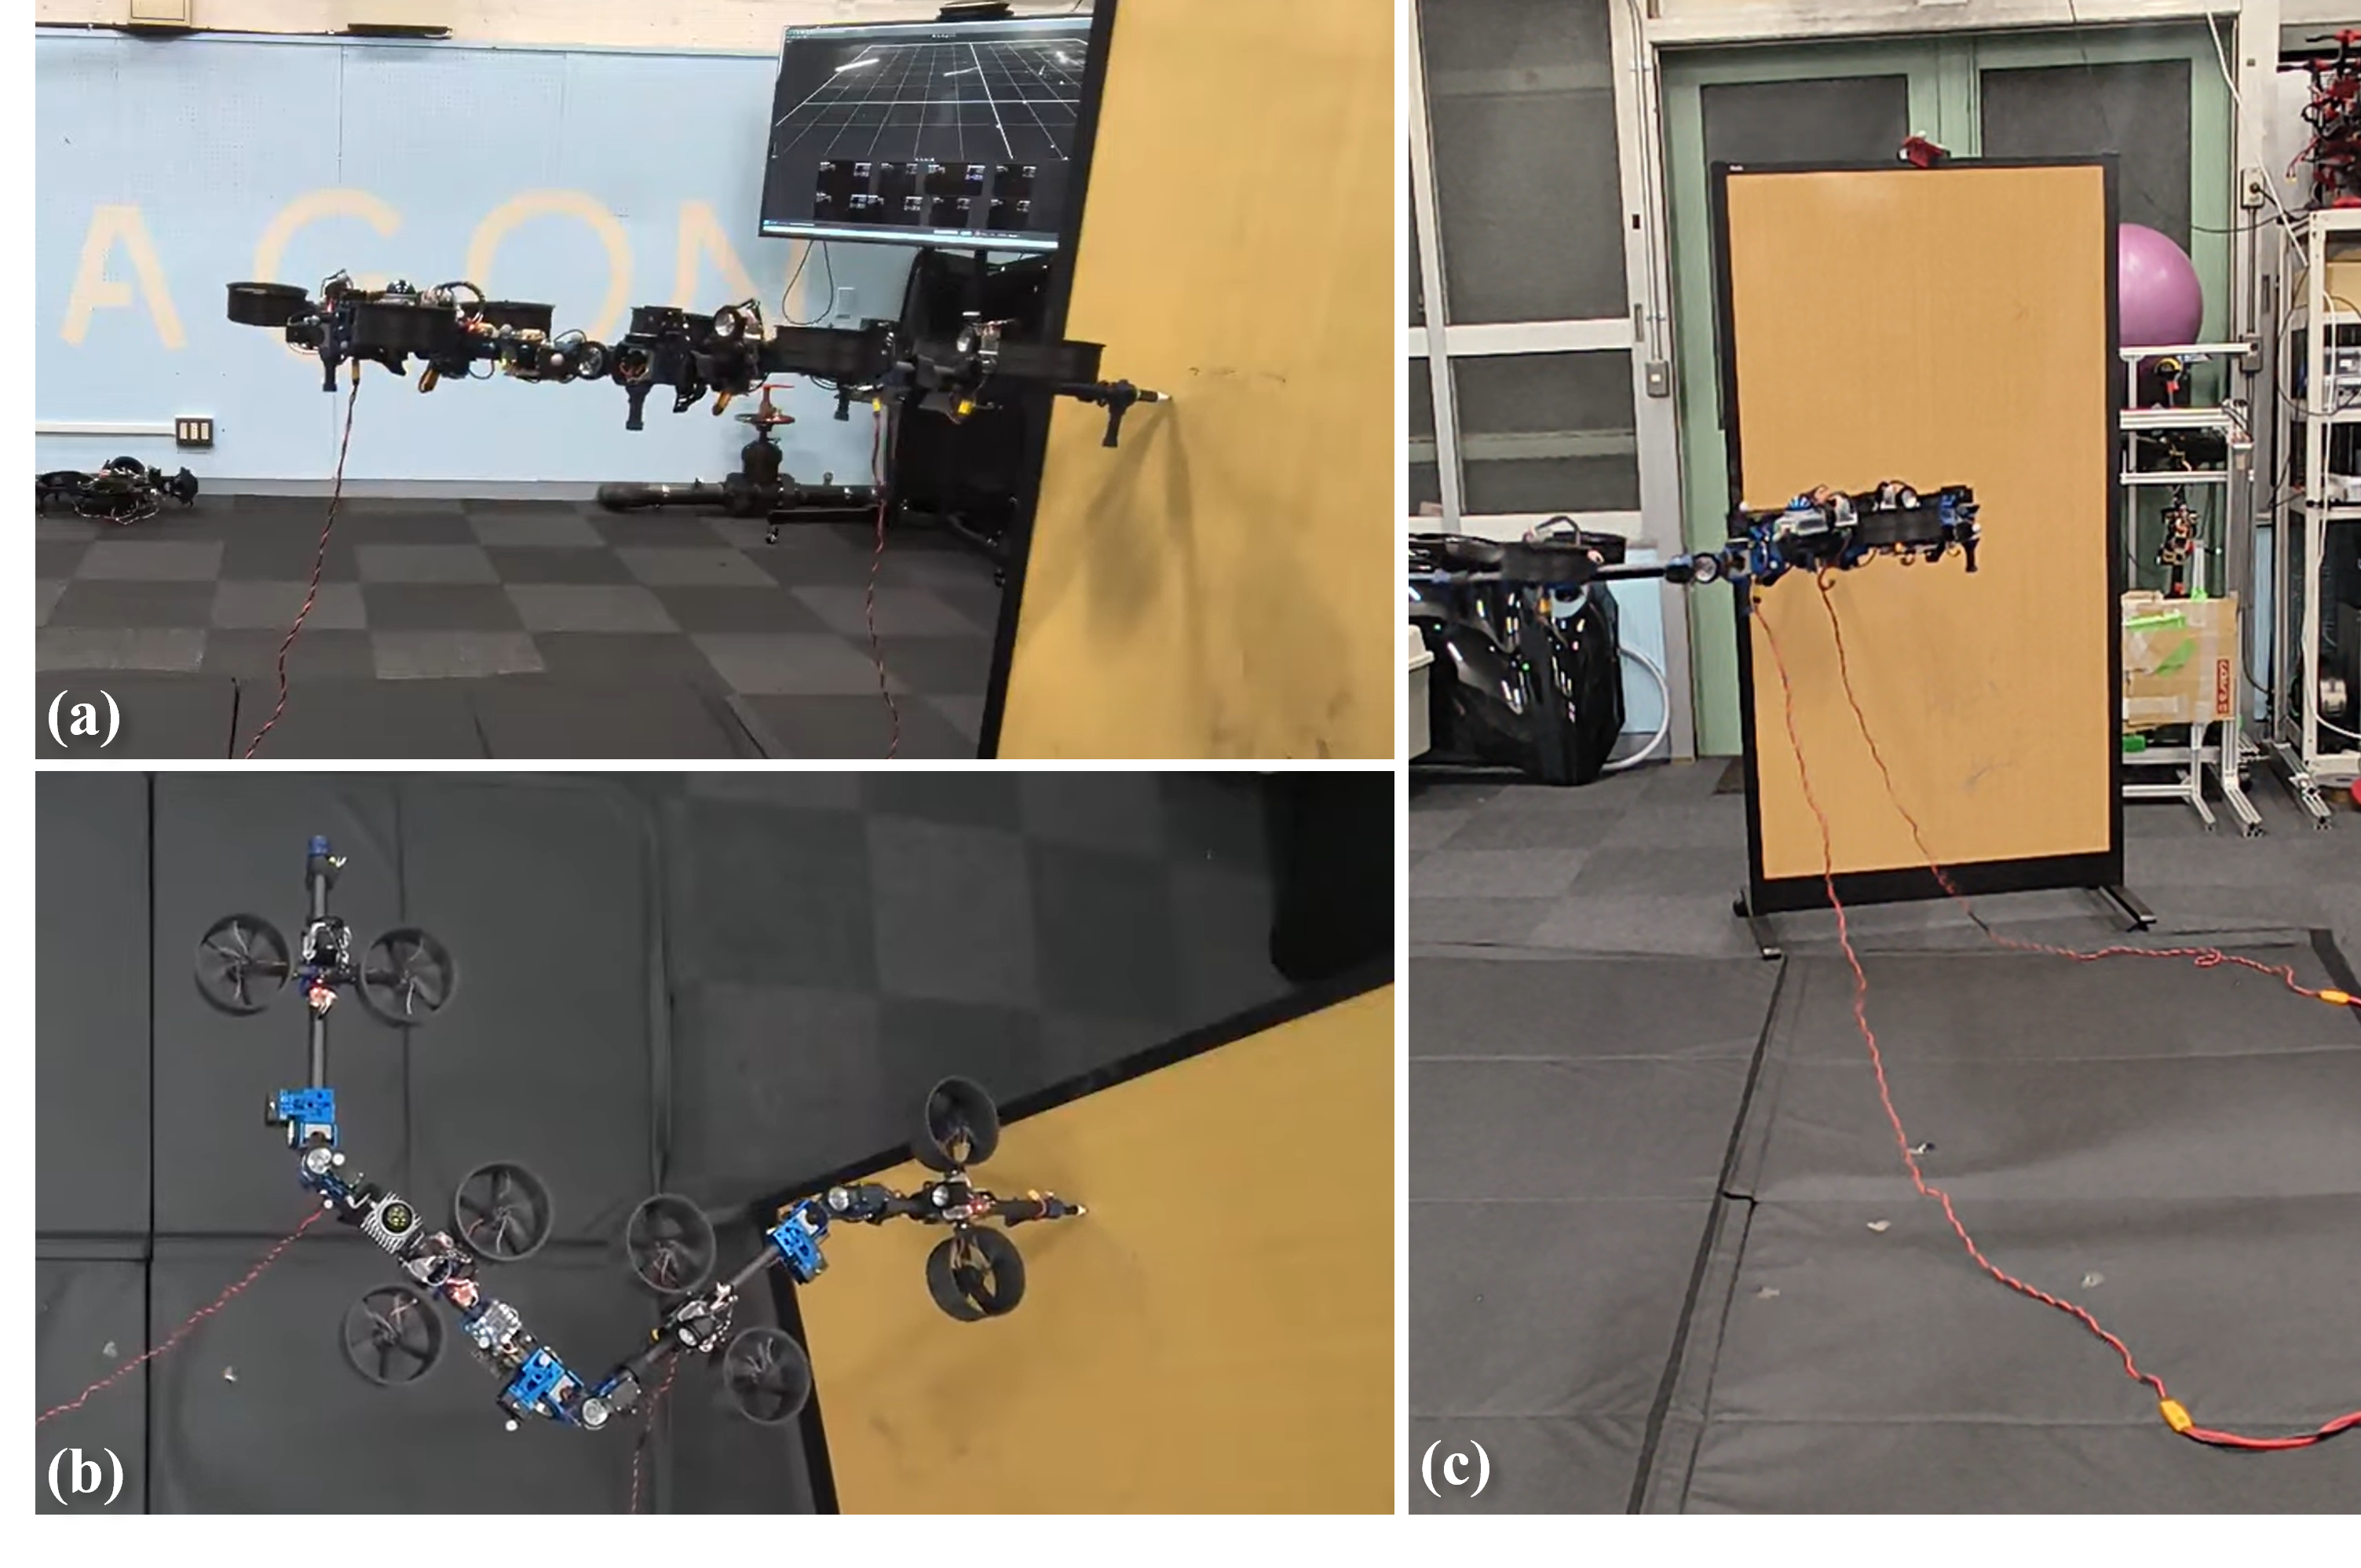
\includegraphics[trim=0 0 0 0,clip,width=\linewidth]
    {figures/chapter6/dragon_experiment.png}}
    \caption{Three view figure of DRAGON in the expeirment. (a) Front view. (b) Side view. (c) Top view.}
    \label{fig:dragon_experiment}
\end{figure}

\begin{figure}[!htbp]
    \centerline{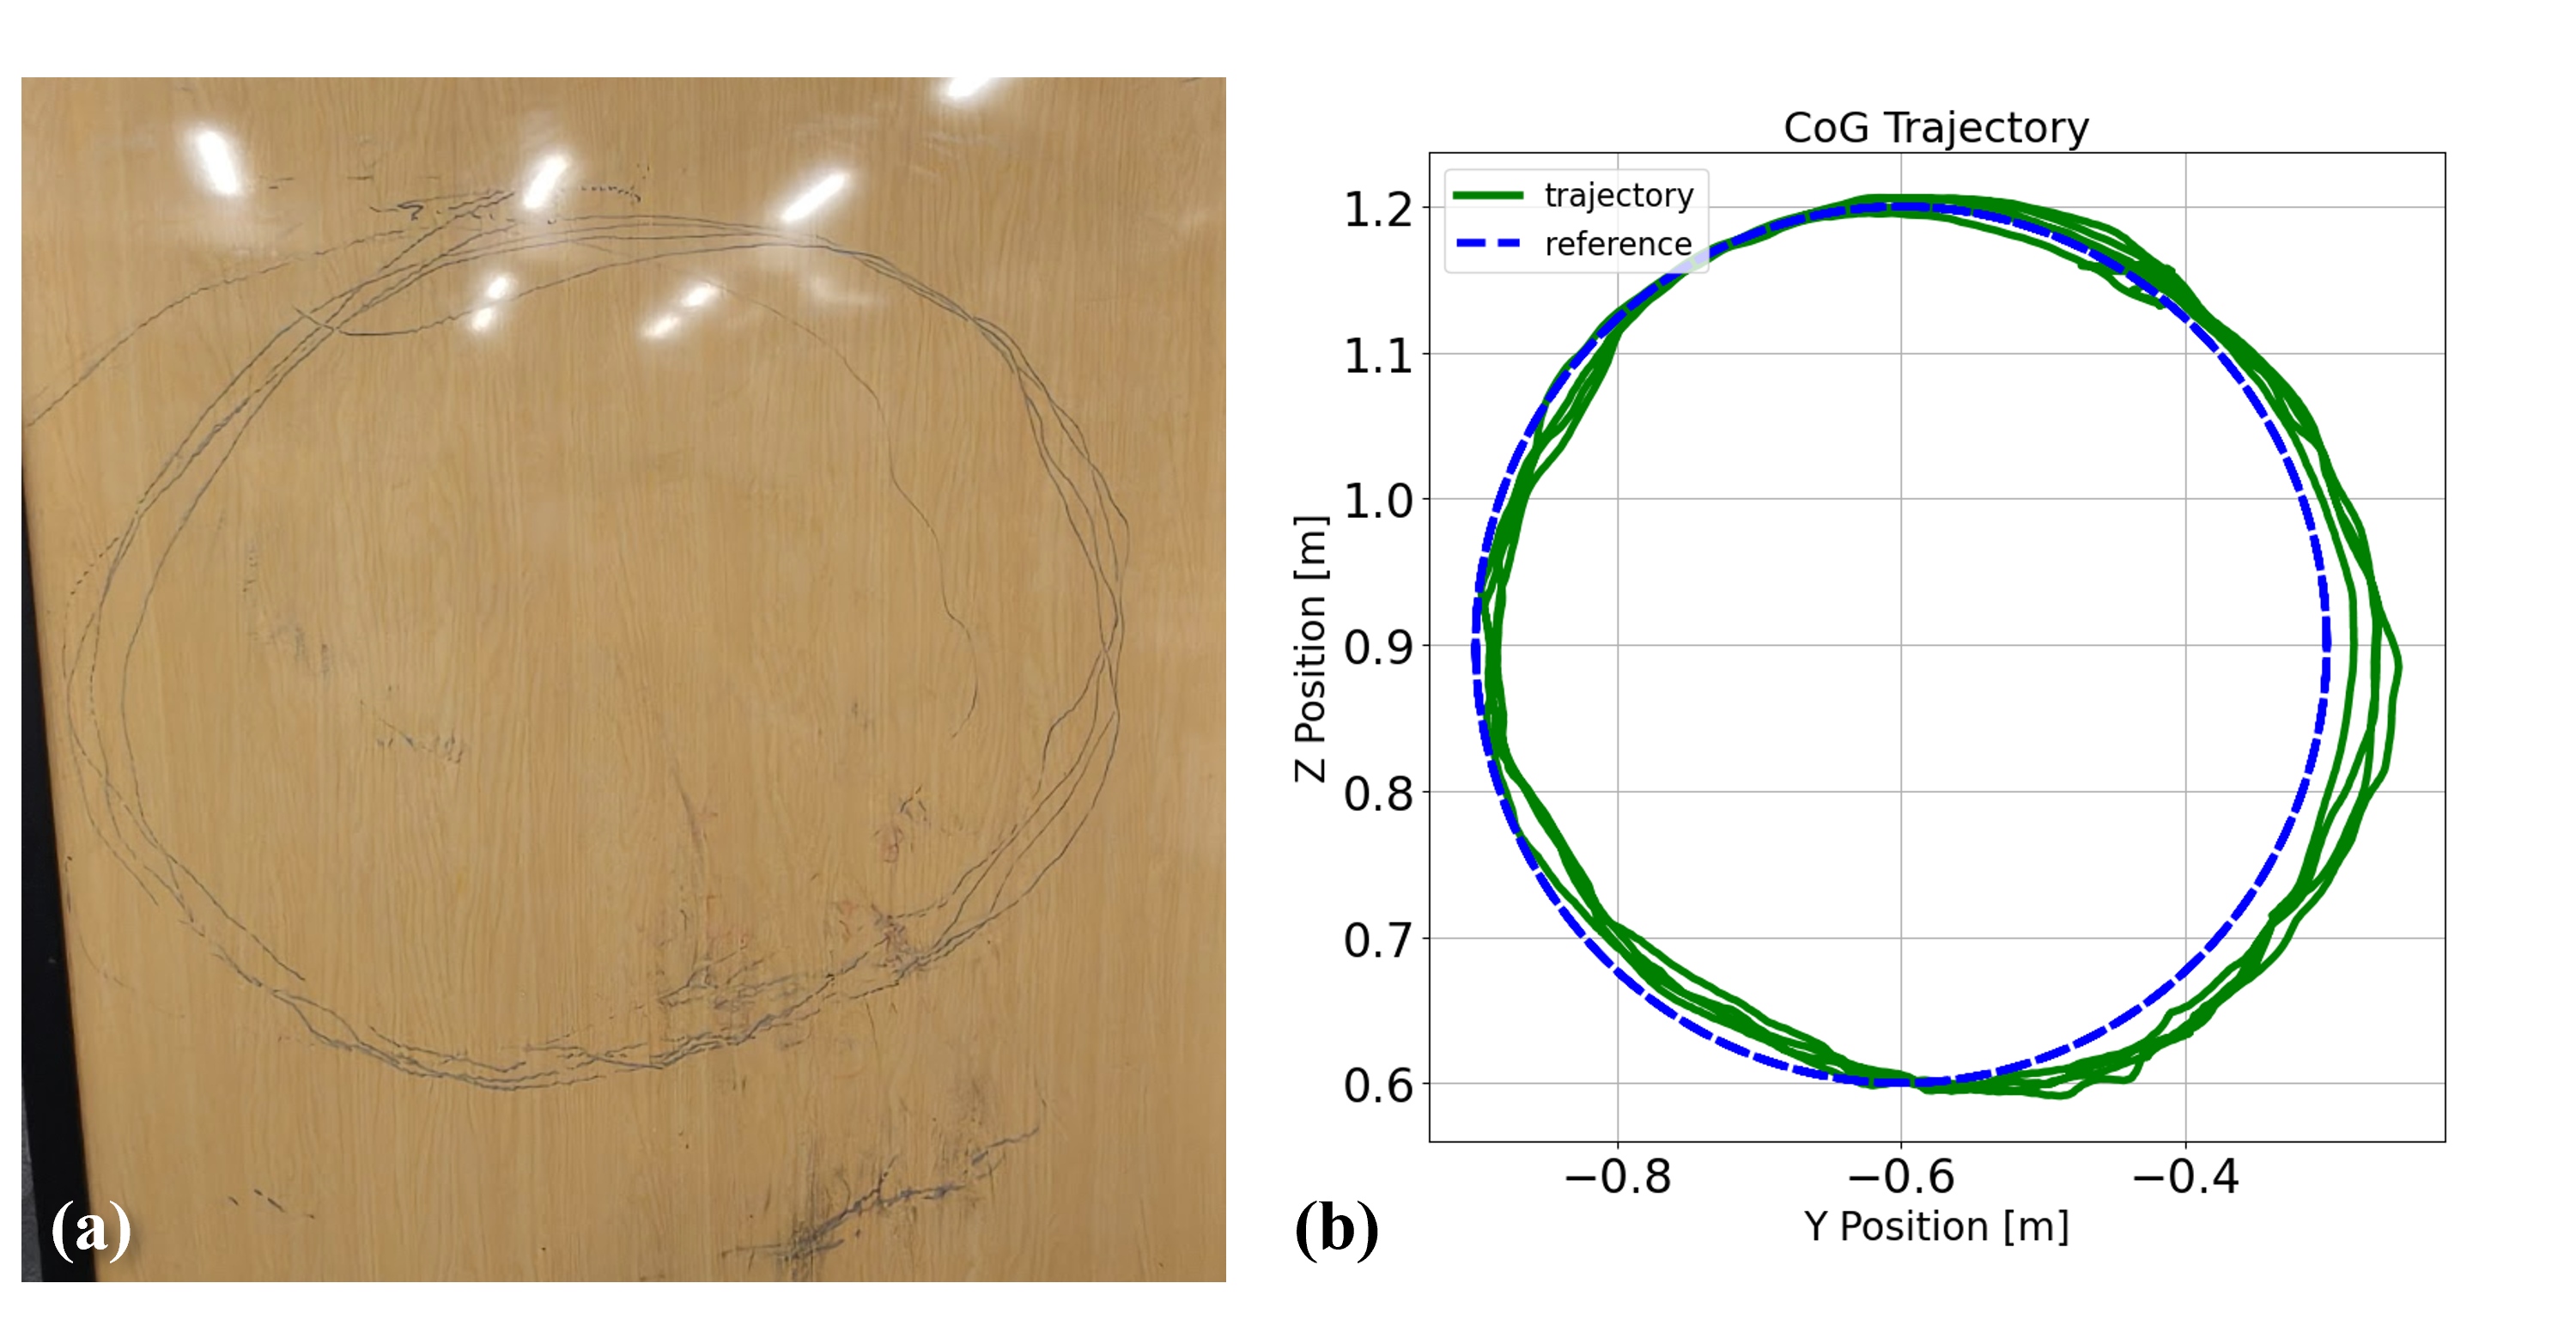
\includegraphics[trim=0 0 0 0,clip,width=\linewidth]
    {figures/chapter6/dragon_trajectory.png}}
    \caption{Three view figure of DRAGON in the expeirment. (a) End effector trajecotry. (b)CoG trajectory.}
    \label{fig:dragon_trajectory}
\end{figure}

\begin{figure}[!htbp]
    \centerline{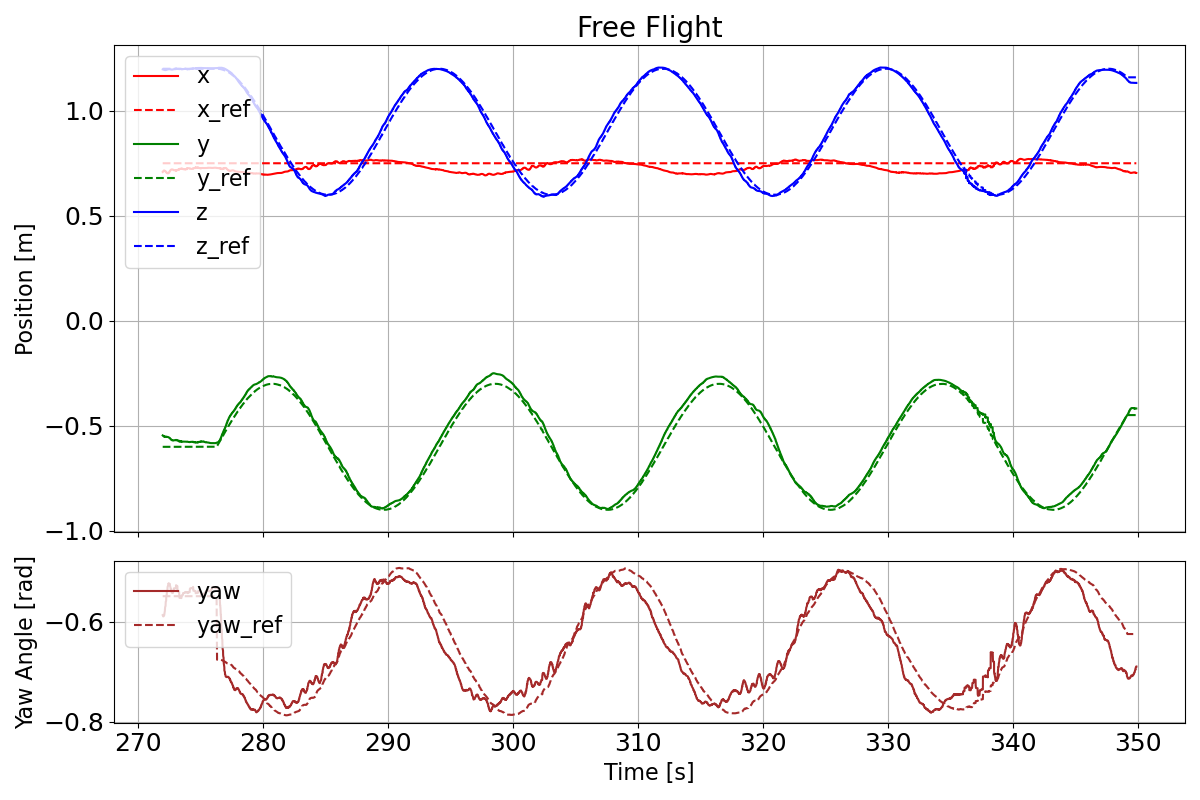
\includegraphics[trim=0 0 0 0,clip,width=\linewidth]
    {figures/chapter6/dragon_plot.png}}
    \caption{Three view figure of DRAGON in the expeirment.}
    \label{fig:dragon_plot}
\end{figure}

\begin{figure}[!htbp]
    \centerline{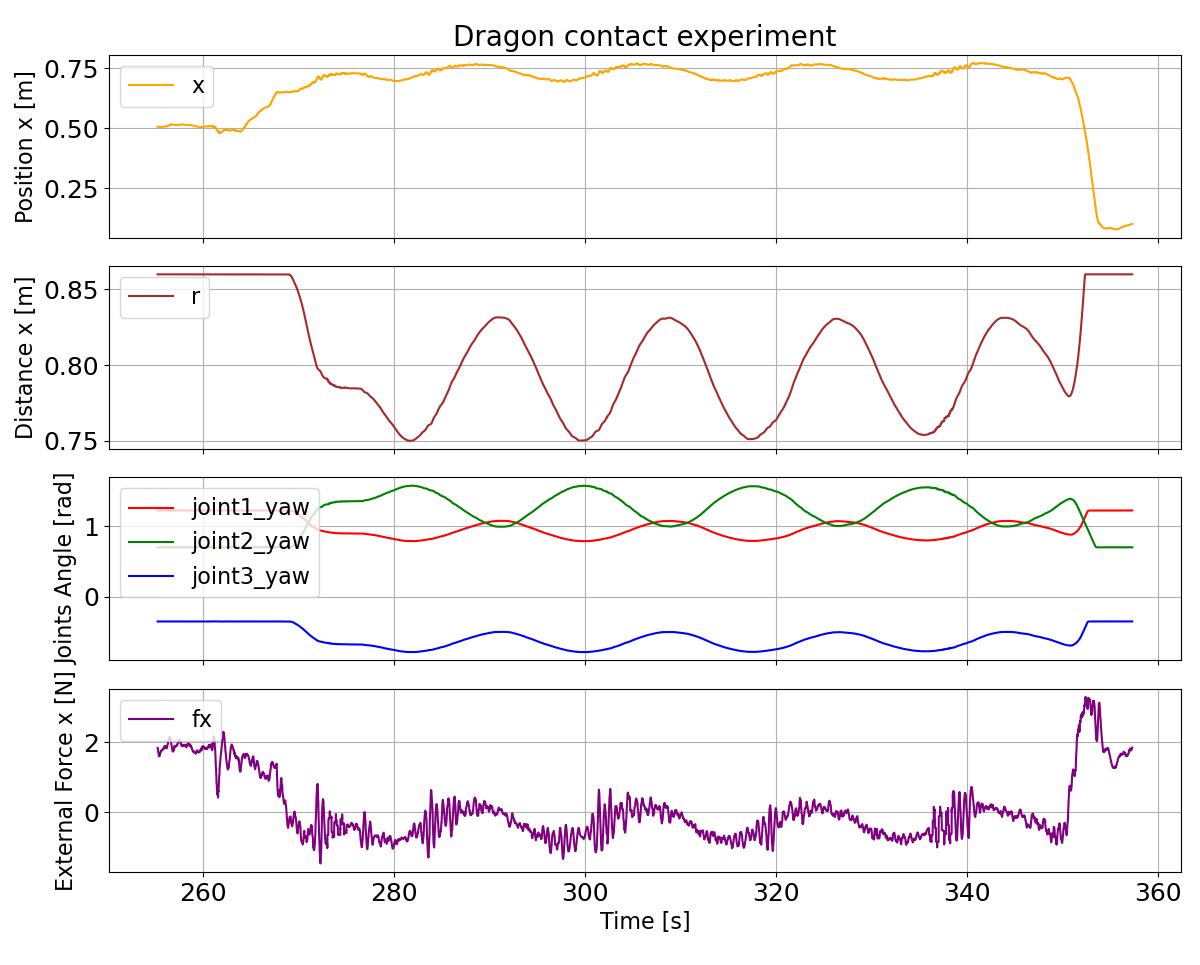
\includegraphics[trim=0 0 0 0,clip,width=\linewidth]
    {figures/chapter6/dragon_contact.png}}
    \caption{Three view figure of DRAGON in the expeirment. }
    \label{fig:dragon_contact}
\end{figure}
and the orientation is required to stay at the initial rotation angle to keep the link4 be vertical with the $y-z$ plane.
%%%%%%%%%%%%%%%%%%%%%%%%%%%%%%%%%%%%%%%%%%%%%%%%%%%%%%%%%%%%%%%%%%%%%%%%%%%%%%%%
\section{Summary}
In this chapter, we show the hybrid impedance-admittance control.